
\section{Introduction}
\label{sec:intro}

\lettrine{T}{raditional} denoising diffusion models are defined on finite-dimension Euclidean spaces \parencite{song2019generative,song2020score,ho2020denoising,nichol2021beatgans}.
Extensions have recently been developed for more exotic distributions, such as those supported on Riemannian manifolds, developed in the previous chapters, and on function spaces of the form \(f:\R^n\to\R^d\)~\parencite{dutordoir2022Neural,kerrigan2022Diffusion,lim2023scorefunction,pidstrigach2023InfiniteDimensional,franzese2023continuous,bond2023infty} i.e. modelling stochastic processes.
In this chapter, we extend diffusion models to further deal with distributions over functions that incorporate non-Euclidean geometry in two different ways.
This investigation of geometry also naturally leads to the consideration of symmetries in these distributions, and as such we also present methods for incorporating these into diffusion models.

Firstly, we look at \emphhypermargin{tensor fields}{def:tensor_field}.
Tensor fields are geometric objects that assign to all points on some manifold a value that lives in some vector space \(V\), approximately functions \(f:\c{M}\to V\).
% Roughly speaking, these are functions of the form \(f: \c{M}\to V\).
These objects are central to the study of physics as they form a generic mathematical framework for modelling natural phenomena.
Common examples include the pressure of a fluid in motion as \(f: \R^3 \to \R\), representing wind over the Earth's surface as \(f: \c{S}^2 \to T\c{S}^2\), \(f\in \Gamma(T\c{S}^2)\), sections of the tangent bundle, or modelling the stress in a deformed object as \(f: \text{Object} \to T\R^3 \otimes T\R^3\), where \(\otimes\) is the \emphhypermargin{tensor product}{def:tensor_product} of the tangent spaces.
Given the inherent symmetry in the laws of nature, these tensor fields can transform in a way that preserves these symmetries.
Leveraging this symmetry can drastically reduce the amount of data required to learn from and reduce training time \cite{elesedy2021provably,elesedy2021provably2,lyle2020benefits,NEURIPS2022_257b9a6a}.


Secondly, we look at functions with manifold codomain, and in particular, at functions of the form \(f: \R \to \c{M}\).
The challenge in dealing with manifold-valued output, arises from the lack of vector-space structure.
In applications, these functions typically appear when modelling processes indexed by time that take values on a manifold.
Examples include tracking the eye of cyclones moving on the surface of the Earth (\cref{sec:cyclone_tracking}), or modelling the joint angles of a robot as it performs tasks \cite{jaquier2021geometry}.

The lack of data or noisy measurements in the physical process of interest motivates a \emph{probabilistic} treatment of such phenomena, in addition to its functional nature.
Arguably the most important framework for modelling stochastic processes are Gaussian processes (GPs) ~\parencite{rasmussen2003gaussian}, as they allow for exact or approximate posterior prediction \parencite{titsias2009Variational,rahimi2007random,wilson2020efficiently}.
These can be viewed as generalisations of the typical multivariate Gaussian distribution, specified by a mean and covariance kernel.
In particular, when choosing equivariant mean and kernel functions, Gaussian processes are invariant to the symmetries their mean and kernel function encode (this is commonly referred to as `stationary') \parencite{terenin22, holderrieth2021equivariant, azangulov2023stationary, azangulov2023stationary2}.
Their limited modelling capacity and the difficulty in designing complex, problem-specific kernels motivated the development of neural processes (NPs)~\cite{garnelo2018neural}, which learn to approximately model a conditional stochastic process directly from data.
Neural processes have been extended to model translation invariant (scalar) processes \parencite{gordon2019Convolutional} and more generic \(\groupE{}\)-invariant processes \parencite{holderrieth2021equivariant}.
In this chapter, we develop geometric diffusion neural processes which incorporate non-Euclidean geometry prior into functional diffusion models.

% Our contributions are three-fold: \begin{enumerate}[label=(\alph*)] \item We incorporate group invariance of the distribution of the generative model by enforcing the covariance kernel and the score network to be group equivariant.
% 	\item We propose a novel Langevin dynamics scheme for efficient conditional sampling. This is independent of the geometric modelling contributions.
% \end{enumerate}

In this chapter we develop two sets of contributions.
Firstly, we produce a framework for placing score-based generative models on the spaces of tensor fields on manifolds, and on the spaces of paths on manifolds.
We accomplish this by considering the finite marginals of a noising process defined on the infinite dimension space of functions, targeting a Gaussian process as the reference distribution.
We investigate a series of methods of parametrising the score function for such a process.
Finally, we derive the constraints required on the score function to ensure that the modelled density is invariant, or if we are modelling a conditional distribution, equivariant.

Secondly we design a new series of conditioning methods to sample the posterior distribution of a prior diffusion model, conditioned on a partial observation.
This method relies on exploiting a decomposition of the score function and an application of Langevin dynamics.
We explore a series of hyperparameter settings for this algorithm, trading off sampling cost with sample quality.

Finally, we empirically evaluate these methods on a series of experimental tasks.

% \section{Background}
% \label{sec:background}

% \textbf{Denoising diffusion models.}
% We briefly recall here the key concepts behind diffusion models on \(\R^d\) and refer the readers to \cite{song2020score} for a more detailed introduction.
% We consider a forward \emph{noising} process \((\v{Y}_t)_{t \geq 0}\) defined by the following Stochastic Differential Equation (SDE) \begin{equation}\label{eq:forward_SDE_dupref} \mathrm{d} \v{Y}_t = -\tfrac{1}{2} \v{Y}_t \mathrm{d} t + \mathrm{d} \v{B}_t,\quad \v{Y}_0 \sim p_0 , \end{equation} where \((\v{B}_t)_{t \geq 0}\) is a \(d\)-dimensional Brownian motion and \(p_0\) is the data distribution.
% The process \((\v{Y}_t)_{t \geq 0}\) is simply an Ornstein--Ulhenbeck (OU) process which converges with geometric rate to \(\mathrm{N}(0,\m{I})\).
% Under mild conditions on \(p_0\), the time-reversed process \((\bar{\v{Y}}_t)_{t \geq 0} = (\v{Y}_{T-t})_{t \in \cbr{0,T}}\) also satisfies an SDE \parencite{cattiaux2021time,haussmann1986time} given by \begin{equation} \mathrm{d} \bar{\v{Y}}_t = \{ \tfrac{1}{2} \bar{\v{Y}}_t + \nabla \log p_{T-t}(\bar{\v{Y}}_t)\} \mathrm{d} t + \mathrm{d} \v{B}_t,\quad \bar{\v{Y}}_0 \sim p_T, \label{eq:backward_SDE_dupref} \end{equation} where \(p_t\) denotes the density of \(\v{Y}_t\).
% Unfortunately we cannot sample exactly from (\ref{eq:backward_SDE_dupref}) as \(p_T\) and the scores \((\nabla \log p_t)_{t\in[0,T]}\) are unavailable.
% First, \(p_T\) is substituted with the limiting distribution \(\mathrm{N}(0,\m{I})\) as it converges towards it (with geometric rate).
% Second, one can easily show that the score \(\nabla \log p_t\) is the minimiser of \(\ell_t(\mathbf{s}) = \E\sbr{\norm{\mathbf{s}(\v{Y}_t) - \nabla_{y_t} \log p_{t|0}(\v{Y}_t|\v{Y}_0)}^2}\) over functions \(\mathbf{s}: \cbr{0,T} \times \R^d \to \R^d\) where the expectation is over the joint distribution of \(\v{Y}_0,\v{Y}_t\), and as such can readily be approximated by a neural network \(\mathbf{s}_\theta(t, y_t)\) by minimising this functional.
% Finally, a discretisation of (\ref{eq:backward_SDE_dupref}) is performed (e.g.\ Euler--Maruyama) to obtain approximate samples of \(p_0\).

% \begin{figure}
% 	\begin{center}
% 		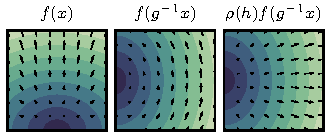
\includegraphics[width=1.\textwidth]{images/geomndp/2d/steerable_demo.pdf}
% 	\end{center}
% 	\caption{Illustration of a vector field \(f: \R^2 \rightarrow \R^2\) being steered by a group element \(g = uh \in \E(2) = \R^2 \rtimes \mathrm{O}(2)\).}
% 	\label{fig:steerable_demo}
% \end{figure}
% \textbf{Steerable fields.}
% In the following we focus on \(G\) being the Euclidean group \(\groupE{}\), that is the set of rigid transformations in Euclidean space.
% Its elements \(g \in \groupE{}\) admits a unique decomposition \(g=uh\) where \(h \in \groupO{d}\) is a \(d\times d\) orthogonal matrix and \(u \in \groupT{}\) is a translation which can be identified as an element of \(\R^d\); for a vector \(x \in \R^d,\)\ \(g\cdot x = h x + u\) denotes the action of \(g\) on \(x\), with \(h\) acting from the left on \(x\) by matrix multiplication.
% This special case simplifies the presentation, but can be extended to the general case is discussed in \cref{sec:manifold_valued_input}.

% We are interested in learning a probabilistic model over functions of the form \(f : \c{X} \rightarrow \R^d\) such that a group \(G\) acts on \(\c{X}\) and \(\R^d\).
% We call a feature field a tuple \((f, \rho)\) with \(f : \c{X} \rightarrow \R^d\) a mapping between input \(x \in \c{X}\) to some feature \(f(x)\) with associated representation \(\rho: G \rightarrow \mathrm{GL}(\R^d)\)~\parencite{scott1996linear}.
% This feature field is said to be \(G\)-steerable if it is transformed for all \(x \in \c{X}, g \in G\) as \( \label{eq:steerable_feature_field} g \cdot f(x) = \rho(g) f(g^{-1} \cdot x).
% \)
% In this setting, the action of \(\groupE{} = \groupT{} \rtimes \groupO{d}\) on the feature field \(f\)  given by \eqref{eq:steerable_feature_field} yields \(g \cdot f(x) = (uh) \cdot f(x) \triangleq \rho(h) f\left(h^{-1} (x -p)\right)\).
% Typical examples of feature fields include scalar fields with \(\rho_{\mathrm{triv}}(g) \triangleq 1\) transforming as \(g \cdot f(x) = f\left(g^{-1} x\right)\) such as temperature fields, and vectors or potential fields with \(\rho_{\mathrm{Id}}(g) \triangleq h\) transforming as \(g \cdot f(x) = h f\left(g^{-1} x\right)\) as illustrated in \cref{fig:steerable_demo}, such as wind or force fields.

% Typically the laws of nature have symmetry, and so we are a priori as likely to see a steerable field in one transformation under the group as another.
% We therefore wish sometimes to build models that place the same density on a field \(f\) as the transformed field \(g \cdot f\).
% Leveraging this symmetry can drastically reduce the amount of data required to learn from and reduce training time.

\section{Geometric neural diffusion processes} \label{sec:euclidean_geom_ndp}

For ease of presentation we begin with our method specialised for tensor fields on Euclidean space.
Later we will generalise this to tensor fields on manifolds.

\subsection{Euclidean tensor fields}
\label{sec:euclidean_tensor_fields}
\begin{figure}
	\begin{center}
		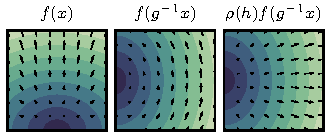
\includegraphics[width=.5\textwidth]{images/geomndp/2d/steerable_demo.pdf}
	\end{center}
	\caption{Illustration of a vector field \(f: \R^2 \rightarrow \R^2\) being steered by a group element \(g = uh \in \E(2) = \R^2 \rtimes \mathrm{O}(2)\).}
	\label{fig:steerable_demo}
\end{figure}
Our aim is to model tensor fields on Euclidean space.
These are an example of a \emphhypermargin{signal on a space}{def:signal}.

Recall that a signal on a space consists of an input space \(X\), a set of symmetries of \(X\), \(G\), and an output space, \(Y\).
We call tuple \((f, \rho)\) with \(f\) as above and \(\rho\) a \emphhyperref{representation}{def:representation} of \(G\), a group action of \(G\) on \(Y\), a \emphmarginnote{feature field}.
Recall the action of \(G\) on a signal is given by 
\[\label{eq:steerable_feature_field}\sbr{g \triangleright f}(x) = \rho(g) f(g^{-1}x), \quad x \in X, \; g\in G.\]

In our setting \(X\) is \(\R^d\), \(Y\) a real vector space, isomorphic to \(\R^{d'}\), and \(G\) the \emphmarginnote{Euclidean group}, the space of rigid symmetries of \(\R^d\).
\(\rho\) is given by the problem being modelled.

The elements \(g \in \groupE[d]{}\) admit a unique decomposition \(g=uh\) where \(h \in \groupO[d]{}\) is a \(d\times d\) orthogonal matrix and \(u \in \groupT[d]{}\) is a translation which can be identified as an element of \(\R^d\); for a vector \(x \in \R^d,\) and \(g = (h, u) \in \groupE[d]{}\), \(g\cdot x = h x + u\) denotes the action of \(g\) on \(x\), with \(h\) acting from the left on \(x\) by matrix multiplication.

The action of \(\groupE[d]{}\) on the feature field \(f\) given by \cref{eq:steerable_feature_field} specialises in this case to \[g \cdot f(x) = (uh) \cdot f(x) \triangleq \rho(h) f\del{h^{-1} (x - u)}.\]
Typical examples of feature fields include scalar fields, \(Y=\R\) with \(\rho_{\mathrm{triv}}(g) \triangleq 1\), such as temperature fields, and vectors fields, \(Y=\R^d\) with \(\rho_{\mathrm{Id}}(g) \triangleq h\), such as wind or force fields.
For an example of a vector field, see \cref{fig:steerable_demo}.

\subsection{Continuous diffusion on function spaces}
\label{sec:functional_diffusion}
We construct a diffusion model on functions \(f: X \rightarrow Y\) by defining a diffusion model for every finite set of marginals.
Most prior works on infinite-dimensional diffusions consider a noising process on the space of functions \parencite{kerrigan2022Diffusion,pidstrigach2023InfiniteDimensional,lim2023score}.
In theory, this allows the model to define a consistent distribution over all the finite marginals of the process being modelled.
In practice, however, only finite marginals can be modelled on a computer and the score function needs to be approximated, and at this step consistency over the marginals is lost.
The only work to stay fully consistent in implementation is \textcite{phillips2022spectral}, at the cost of limiting functions that can be modelled to a finite-dimensional subspace.

With this in mind, we eschew the technically laborious process of defining diffusions over the infinite-dimension space and work solely on the finite marginals following \textcite{dutordoir2022Neural}.
We find that in practice consistency can be well learned from data see, \cref{sec:experiments-gndp}, and this allows for more flexible choices of score network architecture and easier training.

For the modelling problem, we assume that there exists an underlying distribution over tensor fields, \(f \sim \mu\), for \(\mu \in \mathcal{P}(\c{C}({X}, {Y}))\), where \(\mathcal{P}\) is the space of probability measure on the space of continuous functions \(f:X\to Y\).
From this we we have a finite set of observations, observed on a random or static finite index set, that is a dataset
\[
	\del{\del{x_{i, j}, y_{i, j} = f_i(x_{i, j})}_{j=1}^{N_j}}_{i=1}^N, \quad x_{i,j}\in X, \; y_{i,j}\in Y	
\]
for a dataset size \(N\) with \(N_j\) observations per function sample in the dataset.
Examples of this sort of data might include wind observations at sparse weather stations, or pixels making up an image.

It should be noted that a measures on general function spaces \(f: X\to Y\), not just when \(X=\R\), are termed stochastic processes also.
We will refer therefore to the distribution over the data functions as a stochastic process, as well as the stochastic processes defining the forward and reverse stochastic differential equations.

\subsubsection{Noising process}
We denote a stochastic differential equation on the space of functions as \(\del{\v{Y}_t}_{t\geq 0}\)
For a given datapoint \(\del{x_i, y_i}_{i=1}^n = \del{\v{x}, \v{y}}\) of \(n\) observations we denote the noising process on the marginals as \(\del{\v{Y}_t(\v{x})}_{t\geq 0}\) and consider the following forward \emph{noising} process defined by the following multivariate stochastic differential equation 
\[
	\d\v{Y}_t(\v{x}) = \tfrac{1}{2}\beta_t \sbr{\v{m}\del{\v{x}} - \v{Y}_t(\v{x})}\d t + \sqrt{\beta_t} \m{K}(\v{x}, \v{x})^\frac{1}{2} \d \v{B}_t,
	\label{eq:forward_SDE_sp}
\] 
where \(\v{m}(\v{x})_i = m(x_i)\) with \(m: X\to \R\) a mean function and  \(\m{K}(\v{x}, \v{x})_{i, j} = k(x_i, x_j)\) with \(k:X \times X \to \R\) a kernel.
This will converge with geometric rate to \(\c{N}\del{\v{m}\del{\v{x}}, \m{K}\del{\v{x}, \v{x}}}\).
Using the results of \textcite{phillips2022spectral}, this convergence extends to the diffusion on function space \(\v{Y}_t\), which will converge to a Gaussian process with mean function \(m\) and covariance kernel \(k\).
We choose to noise towards a Gaussian process \cite{rasmussen2003gaussian} as they are the function-space generalisation of a multivariate Gaussian.
We hypothesise that by introducing structure into the reference distribution of the diffusion model we can make the sampling process simpler.

In the specific instance where \(k(x_i, x_j) = \delta_{x_i}(x_j)\), then the limiting process \(\v{Y}_\infty\) is simply \emph{white noise}, whilst other choices such as the squared-exponential or Mat\'ern kernel would lead to the associated Gaussian processes.
Note that the \emph{white noise} setting is not covered by the existing theory of functional diffusion models, as a Hilbert space and a square integral kernel are required, see ~\textcite{kerrigan2022Diffusion} for instance.

To draw a sample from \(p_{t|0}(\v{Y}_t(\v{x}) | \v{Y}_0(\v{x}))\) we can sample from the multivariate Gaussian
\[
	\v{Y}_t(\v{x}) &\sim \c{N}\del{\del{1-e^{-\tfrac{1}{2} B(t)}}\v{m}\del{\v{x}} + e^{-\tfrac{1}{2} B(t)} \v{Y}_0(\v{x}), \del{1-e^{-B(t)}}\m{K}(\v{x}, \v{x})} \\&= \c{N}\del{\v{m}_{t|0}(\v{x}), {\sigma}_{t|0}^2 \m{K}(\v{x}, \v{x})}.
\]
where \(B(t) = \int_0^t \beta(s) \d s\).
This can be quickly sampled simply via
\[
	\v{Y}_t(\v{x}) \sim \v{m}_{t|0}(\v{x}) + {\sigma}_{t|0}\v{K}_{t|0}(\v{x}, \v{x})^\frac{1}{2} \v{\varepsilon}, \quad \v\varepsilon\sim\c{N}(0, \v{I}).
\]

The conditional score of the process is given by 
\[ 
	\nabla_{{\v{Y}}_t} \log p_{t}({\v{Y}}_t(\v{x})| \v{Y}_0(\v{x})) = - \v{\Sigma}_{t|0}^{-1} (\v{Y}_t(\v{x}) - \v{m}_{t|0}(\v{x})) = - \sigma_{t|0}^{-1} \v{K}(\v{x}, \v{x})^{-1/2} \varepsilon ,
\] 
allowing for the use of denoising score matching.
See \cref{sec:multivariate_ou} for these results.

\subsubsection{Denoising process}
Using the results presented in \cref{sec:manifold_time_reversal}, the time-reversal process \(({\v{Y}}_t^\vsla{})_{t \geq 0}\) also satisfies a stochastic differential equation, given by 
\[
	\d\v{Y}_t^\vsla{}(\v{x}) = \beta_t \sbr{\tfrac{1}{2}\del{\v{m}\del{\v{x}} - \v{Y}_t(\v{x})} + \m{K}(\v{x}, \v{x}) \nabla\log p^{\v{x}}_{T-t}(\v{Y}_t^\vsla{}(\v{x}))}\d t + \sqrt{\beta_t} \m{K}(\v{x}, \v{x})^\frac{1}{2} \d \v{B}_t,
	\label{eq:backward_SDE_dupref2}\nonumber
\] 
with \(p^{\v{x}}_t\) the density of \(\v{Y}_t(\v{x})\) w.r.t.~the Lebesgue measure.
In practice, the Stein score \(\log p_{T-t}\) is not tractable and is approximated by a neural network.
We then consider the generative stochastic process model defined by first sampling with \(\v{Y}_0^\vsla{} \sim \c{N}\del{\v{m}\del{\v{x}}, \m{K}(\v{x}, \v{x})}\) and then simulating the reverse diffusion \eqref{eq:backward_SDE_dupref2} (e.g. via Euler-Maruyama discretisation).


\subsubsection{Score parametrisation and training loss}
As the reverse stochastic differential equation \eqref{eq:backward_SDE_dupref2} involves the preconditioned score \(\m{K}(\v{x}, \v{x}) \nabla\log p_{t}\), we directly approximate it with a neural network \((\v{Ks})_\theta: [0, T] \times {X}^n \times {Y}^n \rightarrow T {Y}^n\).

We learn the preconditioned score \((\v{Ks})_\theta\) by minimising the following denoising score matching (DSM) loss~\parencite{Vincent2010} weighted by \(\Lambda(t)\) \begin{align}  \mathcal{L}(\theta; \Lambda(t)) \nonumber&= \mathbb{E} [\| \v{s}_\theta(t, \v{Y}_t) - \nabla \log p_{t}({\v{Y}}_t| \v{Y}_0)\|_{\Lambda(t)}^2 ] \\ &= \mathbb{E} [ \| \sigma_{t|0}\cdot (\v{Ks})_\theta(t,\v{Y}_t) + \v{K}(\v{x}, \v{x})^{1/2} \varepsilon \|_2^2 ] ,\label{eq:loss}  \end{align} with \(\Lambda(t)  = \sigma_{t|0}^2\v{K}(\v{x}, \v{x})^\top \v{K}(\v{x}, \v{x})\) where \(\|x\|^2_\Lambda = x^\top \Lambda x\).
Note that when targeting a unit-variance white noise, \(k(x_i, x_j) = \delta_{x_i}(x_j)\), the loss \eqref{eq:loss} reverts to the denoising score matching loss with weighting \(\lambda(t)=1/\sigma_{t|0}^2\)~\parencite{song2020score}.

In \cref{sec:app_parameterisation} we explore several preconditioning terms and associated weighting \(\Lambda(t)\).
Overall, we found the preconditioned score \(\v{K}(\v{x}, \v{x}) \nabla \log p_t\) parameterisation, in combination with the above loss, to perform best, as shown by the ablation study in \cref{fig:app:score-parametrization-ablation}.

\subsubsection{A discussion on model consistency}
\label{sec:consistency}
So far we have defined a generative model over functions via distributions over sets of finite marginals \(\v{Y}_0(\v{x})\).
These finite marginals arise from a stochastic process if, as per the Kolmogorov extension theorem \parencite{oksendal2003stochastic}, they satisfy \emph{exchangeability} and \emph{consistency} conditions.

Exchangeability can be satisfied by parametrising the score network such that the score network is equivariant with respect to permutation, i.e. \(\mathbf{s}_\theta(t, \sigma \circ x, \sigma \circ {y}) = \sigma \circ \mathbf{s}_\theta(t, x, {y})\) for any \(\sigma \in \Sigma_n\).

Additionally, we have that the forward noising processes on the marginals \(({\v{Y}}_t^\vsra{}(\v{x}))_{\v{x} \in \c{X}}\), where \(\c{X}\) is the set of all finite index sets trivially consistent for any \(t \in \R_+\) since these are the marginals of a stochastic process as per \cref{prop:mOU}.
Consequently, so is the (true) time-reversal marginals \(({\v{Y}}_t^\vsla{}(\v{x}))_{\v{x} \in \c{X}}\).

When approximating the score \(\mathbf{s}_\theta \approx \nabla \log p_{t}\) however, we lose the consistency over the generative process \({\v{Y}}_t^\vsla{}(x)\) as the constraint on the score network is non-trivial to satisfy.
The consistency constraint is very strong constraint on the model class, and as soon as one goes beyond linearity (of the posterior with respect to the context set), it is non-trivial to enforce without directly parameterising a stochastic process, e.g. as \textcite{phillips2022spectral} do.
We therefore avoid this and aim to learn consistency from data.
Empirically there seems to be a strong trade-off between satisfying consistency, and the model's ability to fit complex process and scale to large datasets.

\subsection{Invariant and equivariant geometric neural diffusion processes}

So far the model defined does not build in any symmetries desired.
In this section we show how we can incorporate such symmetries.
In particular, we aim to incorporate the symmetries of tensor fields as described in \cref{sec:euclidean_tensor_fields}.

\subsubsection{Invariant stochastic processes}
Let \(\del{F, \sigalg{F}}\) be a measurable space, and let \(G\) be a group with a group action on \(F\).
Let \(\Lambda_F\) be the space of probability measures on \(F\).
For \(\mu \in \Lambda_F\) we define the action of \(G\) on \(\mu\) via the measurable sets of \(\sigalg{F}\) as 
\[
	\sbr{g\cdot \mu}(\rm{F}) = \mu(g^{-1}\cdot \rm{F}) = \mu(\cbrcolon{g^{-1}\cdot f}{f\in \rm{F}})
\]
for \(g\in G\), \(\rm{F}\in \sigalg{F}\).
This action implies
\[
	\sbr{g\cdot \mu}(g\cdot \rm{F}) = \mu(\rm{F})
\]
for \(g\in G\), \(\rm{F}\in \sigalg{F}\).

A probability measure \(\mu\) on \(F\) is said to be \emphmarginnote{\(G\)-invariant measure} if
\[
	g\cdot \mu = \mu \as
\]
This definition naturally covers stochastic processes of the form we are studying with \(F\) as a space of function.
In the Gaussian process literature an invariant Gaussian process is often termed as a `stationary' stochastic process.

Let \(\nu\) be a measure on sets of finite marginal, that is it a distribution on sets \((x_1, ..., x_n)\) for variable \(n\) and randomly generates sets of marginals to evaluate the stochastic process on.
Assume this is invariant under the group action \(g \cdot (x_1, ..., x_n) = (g\cdot x_1, ..., g\cdot x_n)\).
The invariances of \(\mu\) and \(\nu\) together mean that for a given set of observations of the stochastic process, \(\del{\v{x}, \v{y}} = \del{\cbr{x_i}_{i=1}^n, \cbr{y_i=f(x_i)}_{i=1}^n}\) for \(f\sim \mu\) and \(\v{x}\sim \nu\), we are as likely to see this observation as we are to see the transformed observations \(g \cdot \del{\v{x}, \v{y}}\).
The transformation of observations is defined in the Euclidean tensor field case by \[g \cdot \del{\v{x}, \v{y}} = \del{\cbr{g \cdot x_i}_{i=1}^n, \cbr{\rho(h) y_i}_{i=1^n}}\label{eq:sample_transform_euclidean},\]
where \(\rho\) is a representation of \(\groupO[d]{} \subset G\).
We aim therefore to define a model that preserves this \(G\)-invariance.

\subsubsection{Invariant diffusion processes}
First, we recall such a necessary and sufficient condition for Euclidean Gaussian processes to be invariant.
\begin{proposition}[Invariant (stationary) Gaussian process \parencite{holderrieth2021equivariant}]
	\label{prop:inv_gp}
	We have that a Gaussian process \(\mathrm{GP}(m, k)\) is \(G\)-invariant if and only if its mean \(m\) and covariance \(k\) are suitably \(G\)-equivariant---that is, for all \(x,x' \in \c{X}, g \in G\) \begin{align} m(g \cdot x) = \rho(g) m(x) \ \ \text{ and } \ \ k(g \cdot x, g \cdot x') = \rho(g) k(x, x') \rho(g)^\top.
	\end{align}
\end{proposition}

Trivial examples of \(\groupE{}\)-equivariant kernels include diagonal kernels \(k = k_0 \m{I}\) with \(k_0\) invariant~\parencite{holderrieth2021equivariant}, but see \cref{sec:app_vec_gp} for non-trivial instances introduced by \textcite{macedo2010learning}.

Building on \cref{prop:inv_gp}, we then state that our introduced neural diffusion process.
\begin{proposition}[Invariant neural diffusion process~\parencite{yim2023se}]
	\label{prop:inv_prior}
	We denote by \(({\v{Y}}_t^\vsla{}(\v{x}))_{t \in [0, T]}\) the process induced by the time-reversal stochastic differential equation \eqref{eq:backward_SDE_dupref2} on the marginals \(\v{x}\).
	The score is approximated by a score network \[\mathbf{s}_\theta: \sbr{0, T} \times {X}^n \times {Y}^n \rightarrow T {Y}^n\], and the law of the limiting process is given by \[\mathcal{L}({\v{Y}}_0^\vsla{}) \sim \mathrm{GP}(m, k)(\v{x})\], a \(G\)-invariant Gaussian process evaluated on the marginals \(\v{x}\) (\cref{prop:inv_gp}).
	If we additionally assume that the score network is \(G\)-equivariant vector field, i.e. \(\mathbf{s}_\theta(t, g\cdot x, \rho(g) {y}) = \rho(g) \mathbf{s}_\theta(t, x, {y})\) for all \(x \in {X}, g \in G\), then for any \({t \in [0, T]}\) the law of \(\del{\v{Y}_t^\vsla{}(\v{x})}_{\v{x}\in X^n}\) is \(G\)-invariant in the sense that
	\[
		g \cdot \c{L}({\v{Y}}_t^\vsla{}(\v{x})) = \c{L}(\rho(h) {\v{Y}}_t^\vsla{}(g\cdot\v{x})) = \c{L}({\v{Y}}_t^\vsla{}(\v{x}))
	\]
\end{proposition}
This result can be proved in two ways, from the probability flow ordinary differential equation perspective or directly in terms of stochastic differential equation via the Fokker-Planck, see \cref{sec:proof_inv_prior}.

Suitable architectures to produce such equivariant score functions on points include the \(\groupE[n]{}\)-Equivariant Graph Neural Networks of \textcite{satorras2021en}.

\subsubsection{Equivariant posterior maps}
\label{sec:equivariant_posterior}
The invariant model in the previous section defines a model over a stochastic process.
Often in generative modelling we wish to model the \emphmarginnote{conditional distribution} of a stochastic process.
Explicitly learning the conditional distribution is known as \emphmarginnote{amortised conditioning}.
That is, given a partial observation of a sample from \(\mu\), \(\c{C} = \del{\v{x}_c, \v{y}_c} = \del{\cbr{x_{c,i}, y_{c,i} = f(x_{c, i})}}_{i=1}^n, \; f\sim \mu, \; \v{x}_c \sim \nu\), we want to model the conditional measure of \(\mu\) given \(\c{C}\), \(\mu(\cdot | \c{C})\).

When the prior process \(\mu\) is \(G\)-invaraint, the map from the conditioning set to the posterior, \(P: C\mapsto\mu(\cdot | \c{C})\), inherits a symmetry from \(\mu\).
It is \(G\)-equivariant in the sense that \[
P(g \cdot C) = g \cdot P(C) = g \cdot \mu(\cdot | C) \quad\forall\;C, \; g\in G.
\]  
This is equivalent to saying it satisfies \[\mu(g\cdot A | g \cdot \c{C}) = \mu( A | \c{C}) \quad \forall C\; g\in G\; A\in \sigalg{F},\]
and so we could also as that the posterior is \emph{invariant} in this sense.

A version of this statement specialised for Euclidean Gaussian processes was first proved in \textcite{holderrieth2021equivariant}.
We prove a generalisation of that result to measures on tensor fields on general manifolds, \cref{thm:equiv_posterior_maps}.

This implies for a context set \(\c{C} = \del{\v{x}_c, \v{y}_c}\) and a set of observations from the posterior \(\c{O} = \del{\v{x}_o, \v{y}_o}\), \(\v{x}_o \sim \nu\), we are as likely to see the observations \(\c{O}\) given we already observed \(\c{C}\) as we are to see the observation \(g\cdot\c{O}\) given we already observed \(g\cdot\c{C}\).
Consequently we want to define a conditional generative model that respects this invariance.

\subsubsection{Equivariant conditional diffusion processes}
\label{sec:equiv_cond_diff_process}
In order to construct a diffusion model respecting the conditioning equivariance of the posterior we need to construct a score function of the form
\[
	\v{s}_\theta: \sbr{0, T} \x X^{n_o} \x Y^{n_o} \x X^{n_c} \x Y^{n_c} \to TY^{n_o},
\]
where \(n_o\) is the number of new observations we are modelling the distribution on and \(n_c\) is the size of the conditioning set.
This score function takes the conditioning observations as an auxiliary input.

In order to encode the observed invariance in likelihood, it is sufficient to apply a minor extension of \cref{prop:inv_prior}.
The conditional model will be conditionally equivariant if the reference density is invariant and the conditional score function satisfies
\[
	\v{s}_\theta(t, g \cdot \c{O}_t | g \cdot\c{C}) = \rho(h) \v{s}_\theta(t, \c{O} | \c{C})
\] for all context sets \(\c{C}\in X^{n_c}\x Y^{n_c}\), (partially denoised) observation sets \(\c{O}\in X^{n_o}\x Y^{n_o}\), times \(t\in \sbr{0, T}\) and \(g\in G\).

\subsection{Extension to tensor fields on manifolds}
In the previous section we described the construction of symmetry preserving diffusion models for Euclidean tensor fields.
Here we preset how this can be generalised to tensor fields on manifolds.

Significant work has been done on performing convolutions on feature fields on manifolds (a superset of tensor fields on manifolds), core references being \cite{cohen2021equivariant} for the case of homogeneous spaces and \cite{weiler2023equivariant} for more general Riemannian manifolds.
We recommend these as excellent mathematical introductions to the topic and build on them to describe how to formulate diffusion models over these spaces.

\subsubsection{Tensor fields as sections of bundles}
Formally the fields we are interested in modelling are sections \(\sigma\) of associated tensor bundles of the principle \(G\)-bundle on a Riemannian manifold \((M, g)\) for a given \(G\) structure on the manifold.
We shall denote such a bundle \(BM\) and the space of sections \(\Gamma(BM)\).
The goal, therefore, is to model \textit{random elements} \(f\in \Gamma(BM)\) from this space of sections.
For a clear understanding of this definition, please see \textcite[pages 73-95]{weiler2023equivariant} for an introduction suitable to ML audiences.

The symmetries we shall want to preserve are the \emphhypermargin{Riemannian isometries}{} of the manifold, \(\mathsf{Isom}_{(M, g)}\).
Unlike Euclidean symmetries these may not be global symmetries.

Prior work looking at this setting is \textcite{hutchinson2021vector} where they construct kernels for tensor fields on manifolds, allowing for the use of Gaussian processes in this setting.

\subsubsection{Stochastic processes on spaces of sections}
Given we can see sections as maps \(\sigma: M \to BM\), where an element in \(BM\) is a tuple \((m, b)\), \(m\) in the base manifold and \(b\) in the typical fibre, alongside the condition that the composition of the projection \(\operatorname{proj}_i: (m, b)\mapsto m\) with the section is the identity, \(\operatorname{proj}_i \circ \sigma = \operatorname{Id}\) it is clear we can see distribution over sections as stochastic processes with index set the manifold \(M\), and output space a point in the bundle \(BM\), with the projection condition satisfied.
The projection onto finite marginals, i.e.\ a finite set of points in the manifold, is defined as $\pi_{m_1, .
		.., m_n}(\sigma) = (\sigma(m_1), ..., \sigma(m_n))$.

\subsubsection{Noising process}
To define a noising process over these marginals, we can use Gaussian processes defined in \textcite{hutchinson2021vector} over the tensor fields.
The convergence results of \textcite{phillips2022spectral} hold still, and so using these Gaussian processes as noising processes on the marginals also defines a noising process on the whole section.

\subsubsection{Reverse process}
The results of \textcite{cattiaux2021time} are extremely general and continue to hold in this case of stochastic differential equations on the space of sections.
Note we don't actually need this to be the case as we work with the reverse process on the marginals only, which are much simpler objects.
It is good to know that it is a valid process on full sections though should one want to parameterise a score function on the whole section akin to some other infinite-dimension diffusion models.

\subsubsection{Score function}
The last thing to do therefore is parameterise the score function on the marginals.
If we were trying to parameterise the score function over the \textit{whole} section at once (akin to a number of other works on infinite dimension diffusions), this could present some problems in enforcing the smoothness of the score function.
As we only deal with the score function on a finite set of marginals, however, we need not deal with this issue and this presents a distinct advantage in simplicity for our approach.
All we need to do is pick a way of numerically representing points on the manifold and pick a basis for the tangent space of each point on the manifold.
This lets us represent elements from the tangent space as element of Euclidean space, and therefore also elements from tensor space at each point as elements of Euclidean space as well.
This done, we can use the standard Euclidean score-based modelling framework to model these quantities.

\subsubsection{Encoding symmetries}

A general recipe for encoding symmetries into this generalisation is unlikely to be available.
The symmetry acting on sets of observations of sections of tensor bundles on manifolds are more complex than in the Euclidean case.
The generalisation of \cref{eq:sample_transform_euclidean} is given by
\[g \cdot \del{\v{x}, \v{y}} = \del{\cbr{g \cdot x_i}_{i=1}^n, \cbr{\rho(h(g, x_i)) y_i}_{i=1^n}}\label{eq:sample_transform},\]
where \(i\in\mathsf{Isom}_{(M, g)}\) and \(h: \mathsf{Isom}{(M, g)}\x M \to G\) is a function of the global isometry and the specific point \(x_i\).

One case where this simplifies is when there exists an isometric embedding of the manifold into Euclidean space that also preserve the symmetry of the manifold such that the symmetry in the embedding is a subgroup of the Euclidean group.
Examples of this include \(n\)-spheres \(\c{S}^n\), such as the circle and the sphere.
In this case we can use an architecture that is equivariant to Euclidean transformations and project the outputs onto the tangent space of the embedded manifold.

\subsection{Extension to manifold-valued functions}
\label{sec:manifold_valued_output}
So far we have defined our generative model for tensor fields \(f:\c{M} \to Y\) with \({Y} \isom \R^d\).
We now extend our methodology to model functions of the form \(f: X \to \c{M}\) where \(\c{M}\) is a Riemannian manifold.

In this case \(\c{M}\) does not have the vector space structure necessary to define Gaussian processes.
Fortunately we can still target a know distribution independently on each marginal, since this is well-defined, and as such revert to the Riemannian diffusion models introduced in \cref{cpt:riemannian_score_based_models} with \(n\) independent Langevin noising processes 
\begin{equation} \label{eq:forward_SDE_manifold} \mathrm{d} {\v{Y}}_t(x_i) = - \tfrac{1}{2} \beta_t\nabla U({\v{Y}}_t(x_i)) \mathrm{d} t + \sqrt{\beta_t } \mathrm{d} \v{B}_t^\c{M}
\end{equation} applied to each marginal.
Hence, in the limit \(t \rightarrow \infty\), \({\v{Y}}_t(x)\) has density (assuming it exists) which factors as \(\frac{\d p}{\d \mathrm{Vol}_\c{M}^n} \propto \prod_{i=1}^n e^{-U(y_i)}\).

Since the space of this diffusion is the product of finitely many Riemannian manifolds, the time reversal and parametrisation of the score function approaches of \cref{cpt:riemannian_score_based_models} also apply, giving us a ready method to define a diffusion model on paths.

\section{Langevin conditional sampling of diffusion model}
\label{sec:conditional_sampling}

\begin{figure}
	\centering
	\begin{center}
		% \resizebox{0.5\linewidth}{!}{
			\begin{tikzpicture}
				\Large
				\draw [stealth-, line width = .05cm] (0,0) .. controls  (2,-4) and (3.,2) .. (6,0);
				\draw [-stealth, line width = .05cm, tabblue, dashed] (0,0) -- (1.3,-2.3);
				\draw [-stealth, line width = .05cm, tabred, dashed] (1.3,-2.3) -- (1.3,-1.9);
				\draw [-stealth, line width = .05cm, tabred, dashed] (1.3,-1.9) -- (1.3,-1.7);
				\draw [-stealth, line width = .05cm, tabred, dashed] (1.3,-1.7) -- (1.3,-1.4);
				\draw [-stealth, line width = .05cm, tabblue, dashed] (1.3,-1.45) -- (2.8,-1.35);
				\draw [-stealth, line width = .05cm, tabred, dashed] (2.8,-1.35) -- (2.4, -0.9);
				\node [below=0.2cm] at (6,0) {\(p_0\)};
				\node [left=0.0cm] at (0,0) {\(\mathcal{L}(\bar{\v{Y}}_0) = p_T\)};
				\node [left=0.2cm] at (1.3,-2.1) {\(\mathcal{L}(\bar{\v{Y}}_\gamma^0)\)};
				\node [right=0.1cm] at (1.3,-2.) {\(\mathcal{L}(\bar{\v{Y}}_\gamma^1)\)};
				\node [right=0.1cm] at (1.3,-1.65) {\(\cdots\)};
				\node [above=0.05cm] at (1.3,-1.35) {\(p_{\gamma}\)};
				\node [below right=0.1cm] at (2.8,-0.8) {\(\mathcal{L}(\bar{\v{Y}}_{2\gamma}^0)\)};
				\node [right=0.1cm] at (2.6, -0.7) {\(\mathcal{L}(\bar{\v{Y}}_{2\gamma}^1)\)};
				\node [above left=0.05cm] at (2.6, -0.9) {\(p_{2\gamma}\)};
			\end{tikzpicture}
		% }
	\end{center}
	\caption{
		Illustration of Langevin corrected conditional sampling.
		The black line represents the noising process dynamics \((p_t)_{t \in \cbr{0,T}}\).
		The \textcolor{tabblue}{time reversal (i.e.\ predictor)} step, is combined with a \textcolor{tabred}{Langevin corrector} step projecting back onto the dynamics.
	}
	\label{fig:predictor_corrector}
\end{figure}

\emphmarginnote{Conditional sampling}, or posterior sampling, is the problem of sampling from a prior distribution, conditioned on some partial observations, as discussed in \cref{sec:equivariant_posterior} already.
This is a long standing problem in Bayesian machine learning and Bayesian statistics in general.

% There exist several methods to perform conditional sampling in diffusion models such as: replacement sampling, amortisation and conditional guidance.
% Replacement sampling is not exact and do not recover the correct conditional distributions.
% SMC based methods have been proposed to correct this procedure but they suffer from the limitations of SMC and scale poorly with the dimension \parencite{trippe2022Diffusion}.
% On the other hand, amortisation, require the retraining of the score network for each different conditional task which is impractical in our setting where the context length might change.
% Conditional guidance is a popular method in state-of-the-art image diffusion models but does not recover the true posterior distribution.

% Here we propose a new method for sampling from exact conditional distributions of NDPs using only the score network for the joint distribution.
% Using the fact that the conditional score can be written as \(\nabla_x \log p(x|y) = \nabla_x \log p(x, y) - \nabla_x \log p(y) = \nabla_x \log p(x, y)\) we can therefore, for any point in the diffusion time, conditionally sample using Langevin dynamics, following the stochastic differential equation \(\mathrm{d} \v{Y}_s = \tfrac{1}{2} \mathrm{K} \nabla \log p_{T-t}(\v{Y}_s) \mathrm{d} s + \sqrt{\mathrm{K}} \mathrm{d} \v{B}_s\), by only applying the diffusion to the variables of interest and holding the others fixed.
% While we could sample directly at the end time this proves difficult in practice.
% Similar to the motivation of \textcite{song2019generative}, we sample along the reverse diffusion, taking a number of conditional Langevin steps at each time.
% In addition, we apply the forward noising stochastic differential equation to the conditioning points at each step, as this puts the combined context and sampling set in a region that the score function will be well learned in training.
% Our procedure is illustrated in \Cref{alg:conditioning_langevin}.
% In \cref{app:conditional_sampling} we draw links between \textsc{RePaint} of \textcite{lugmayr2022repaint} and our scheme.


Several previous schemes exist for conditional sampling from diffusion models, each with some limitations.
These include: \begin{itemize} \item Replacement sampling \cite{song2020score}, where the reverse likelihood ordinary differential equation or the reverse stochastic differential equation is evolved but by fixing the conditioning data during the rollout.
	      This method does produce visually coherent sampling in some cases, but is not an exact conditional sampling method.
	\item SMC-based methods \cite{trippe2022Diffusion}, which are an exact method up to the particle filter assumption.
	      These can produce good results but can suffer from the usual SMC methods downsides on highly multi-model data such as particle diversity collapse.
	\item The {\textsc RePaint} scheme of \cite{lugmayr2022repaint}.
	      While not originally proposed as an exact sampling scheme, in \cref{sec:app_conditional_sampling} we show that this method is a specific instantiation of our newly proposed method, and is therefore exact.
	\item Amortisation methods, e.g. \textcite{phillips2022spectral} and \cref{sec:equiv_cond_diff_process}.
	      While they can be effective, these methods can never perform exact conditional sampling, by definition, and can take significant model capacity to learn approximate conditioning maps.
\end{itemize}

Our goal in this section is to produce an exact, performant, sampling scheme that does not rely on SMC-based methods.
Instead, we base our method on Langevin dynamics.
For the initial presentation in the section we consider a distribution over a fixed state space, \(\v{x}\in X^n\).
We will adapt this to the setting of modelling the marginals of a stochastic process later.
Consider the setting where we have partially observed \(\v{x}\), \(v{x}^c \in X^{n_c}\), and we wish to sample \(\v{x}^o\in X^{n_o}\), such that \(n_c + n_o = n\).
If we have a score function trained over the state space \(\v{x} = [\v{x}^c, \v{x}^o]\) we exploit the following score breakdown: \[\nabla_{\v{x}^o} \log p(\v{x}^o|\v{x}^c) = \nabla_{\v{x}^o} \log p([\v{x}^o, \v{x}^c]) - \nabla_{\v{x}^o} \log p(\v{x}^c) = \nabla_{\v{x}^o} \log p(\v{x}).\] This means that if we have access to the score on the joint variables, we have access to the conditional score by simply taking the joint score and ignoring  the gradient for the variables we are conditioning on.

In a score-based model we learn the time-dependent score function \(s_\theta(t, \v{x}) \approx \nabla_{\v{x}}\log p_t(\v{x})\).
We could use this to perform Langevin dynamics at \(t=\epsilon\), some time very close to \(0\).
Similar to \cite{song2019generative} however, this produces the twin issues of how to initialise the dynamics, given a random initialisation will start the sampler in a place where the score has been badly learnt, and very slow mixing times for complex distributions, producing inaccurate sampling.

Instead, we follow a scheme of tempered Langevin sampling detailed in \cref{alg:conditioning_langevin}.
Starting at \(t=T\) we sample an initialisation of \(\v{x}^o\) based on the reference distribution.
Progressing from \(t=T\) towards \(t=\epsilon\) we alternate between running a series of inner Langevin corrector steps to sample from the distribution \(p_{t}(\v{x}^o_t | \v{x}^c_t)\), and a single outer backwards stochastic differential equation step to sample from \(p_{t}(\v{x}^o_{t-\gamma} | \v{x}^c_t)\) with a step size \(\gamma\).
At each inner and outer step, we sample a noised version of the conditioning variables \(\v{x}^c_t\) based on the forward stochastic differential equation applying noise to these context points, \(p_{t|0}(\v{x}_t^c | \v{x}^c)\).
For the exactness of this scheme, all that matters is that at the end of the sampling scheme, we are sampling from \(p_{0}(\v{x}^o | \v{x}^c)\).
The rest of the scheme is designed to map from the initial sample at \(t=T\) of \(\v{x}^o\) to a viable sample through \textit{regions where the score has been learnt well}.

We apply this scheme to the problem of sampling from conditional distributions on the marginals of a diffusion model modelling a stochastic process by applying it to a fixed set of marginals at a time.
Consider that we have a set of conditioning observations, \((\v{x}^c, \v{y}^c)\), and a set of index locations we wish to sample conditional observations at, \(\v{x}^o\).
A score-based model on the marginals has learnt the distribution \(\nabla_{\v{y}^c, \v{y}^o}\log p_t^{\v{x}^c, \v{x}^o}(\v{y}^c_t, \v{y}^o_t)\).
We can therefore compute the conditional score
\[
	\nabla_{\v{y}^o_t} \log p_t^{\v{x}^c | \v{x}^o}(\v{y}^c_t| \v{y}^o_t) = \nabla_{\v{y}^o_t} \log p_t^{\v{x}^c \v{x}^o}(\v{y}^c_t, \v{y}^o_t),
\] again by ignoring the gradients of the conditioning variables from the learnt score function.
The algorithm for doing this conditioning is laid out in \cref{alg:conditioning_langevin}.

\begin{algorithm}[t]
	\caption{Conditional sampling with Langevin dynamics.
	}
	\label{alg:conditioning_langevin}
	\small
	\begin{algorithmic}
		\State {\bfseries Require:}
		Score network \(\mathbf{s}_\theta(t, \v{x}, \v{y}) \), \textcolor{algcol}{conditioning points \((\v{x}^c, \v{y}^c)\)}, query locations \(\v{x}^o\) \State \({\v{x}} = \sbr{\textcolor{algcol}{\v{x}^c}, \v{x}^o}\) \Comment{Augmented inputs set} \State \({\v{y}}_T^o \sim \c{N}(\v{m}(\v{x}^o), \v{K}(\v{x}^o,\v{x}^o))\) \Comment{Sample initial noise} 
		\For{$t \in \cbr{T, T- \gamma, .
						.., \epsilon}$}
			\State \(\textcolor{algcol}{\v{y}^c_t \sim p_{t|0}^{\v{x}^c}(\cdot | \v{y}^c)}\) \Comment{Sample context noise from forward SDE} 
			\State \(Z \sim \c{N}(0, \m{I})\) \Comment{Sample tangent noise}
			\State \( \sbr{\textunderscore, {\v{y}}_{t-\gamma}^o} = \sbr{\textcolor{algcol}{\v{y}^c_t}, {\v{y}}_t^o} + \gamma \left\{ -\frac{1}{2} \left( m(\bar{\v{x}}) - \sbr{\textcolor{algcol}{\v{y}^c_t}, {\v{y}}_t^o} \right) + \mathrm{K}(\bar{\v{x}}, \bar{\v{x}}) \mathbf{s}_\theta(t, \bar{\v{x}}, \sbr{\textcolor{algcol}{\v{y}^c_t}, {\v{y}}_t^o}) \right\} + \sqrt{\gamma} \mathrm{K}({\v{x}}, {\v{x}})^{1/2}
			Z \) \Comment{Euler-Maruyama step} 
			\For{\(l \in \{1, \dots, L \}\)} 
					\State \(\textcolor{algcol}{\tilde{\v{y}}^c_{t-\gamma} \sim p_{t-\gamma}^{\v{x}^c}(\cdot | \v{y}^c_0)}\) \Comment{Sample context noise from forward SDE} 
					\State \(Z \sim \c{N}(0, \m{I})\) \Comment{Sample tangent noise} 
					\State \( \sbr{\textunderscore, \tilde{\v{y}}_{t-\gamma}^o} = \sbr{\textunderscore, \tilde{\v{y}}_{t-\gamma}^o} + \frac{\gamma}{2} \mathrm{K}(\bar{\v{x}}, \bar{\v{x}}) \mathbf{s}_\theta(t-\gamma, \bar{\v{x}}, \sbr{\textcolor{algcol}{\v{y}^c_{t-\gamma}}, \tilde{\v{y}}_{t-\gamma}^*}) + \sqrt{\gamma} \mathrm{K}({\v{x}}, {\v{x}})^{1/2} Z \) \Comment{Langevin step} 
				\EndFor 
			\State \( \v{y}_{t-\gamma}^o = \tilde{\v{y}}_{t-\gamma}^*\) 
		\EndFor
	\State {\bfseries return} \({\v{y}}_\epsilon^o\) 
	\end{algorithmic}
\end{algorithm} 

% Instead, we follow a scheme of tempered Langevin sampling detailed in \cref{alg:conditioning_langevin}.
% Starting at \(t=T\) we sample an initialisation of \(\v{y}^o\) based on the reference distribution.
% Progressing from \(t=T\) towards \(t=\epsilon\) we alternate between running a series of Lavgevin corrector steps to sample from the distribution \(p_{t, \v{x}^o}(\v{y}^o | \v{y}^c)\), and a single backwards SDE step to sample from \(p_{\v{x}}(\v{y}_{t-\gamma} | \v{y}_t)\) with a step size \(\gamma\).
% At each inner and outer step, we sample a noised version of the conditioning points \(\v{y}^c\) based forward SDE applying noise to these context points, \(p_{t, \v{x}^c}(\v{y}_t^c | \v{y}^c)\).
% For the exactness of this scheme, all that matters is that at the end of the sampling scheme, we are sampling from \(p_{\v{x}^o}(\v{y}^o | \v{y}^c)\) (up to the \(\epsilon\) away from zero clipping of the SDE).
% The rest of the scheme is designed to map from the initial sample at \(t=T\) of \(\v{y}^o\) to a viable sample through \textit{regions where the score has been learnt well}.

\subsection{Noising schemes}

Given the noising scheme applied to the context points does not actually play into the theoretical exactness of the scheme, only the practical difficulty of staying near regions of well-learnt score, we could make a series of different choices for how to noise the context set at each step.

The choices that present themselves are \begin{enumerate} 
	\item The initial scheme of sampling context noise from the forward stochastic differential equation every inner and outer step.
	\item Only re-sampling the context noise every outer step, and keeping it fixed to this for each inner step associated with the outer step.
	\item Instead of sampling independent marginal noise at each outer step, sampling a single noising trajectory of the context set from the forward SDE and use this as the noise at each time.
	\item Perform no noising at all.
	      Effectively the replacement method with added Langevin sampling.
\end{enumerate}
These are illustrated in \cref{fig:noise_schemes}.
\begin{figure}[t]
	\centering
	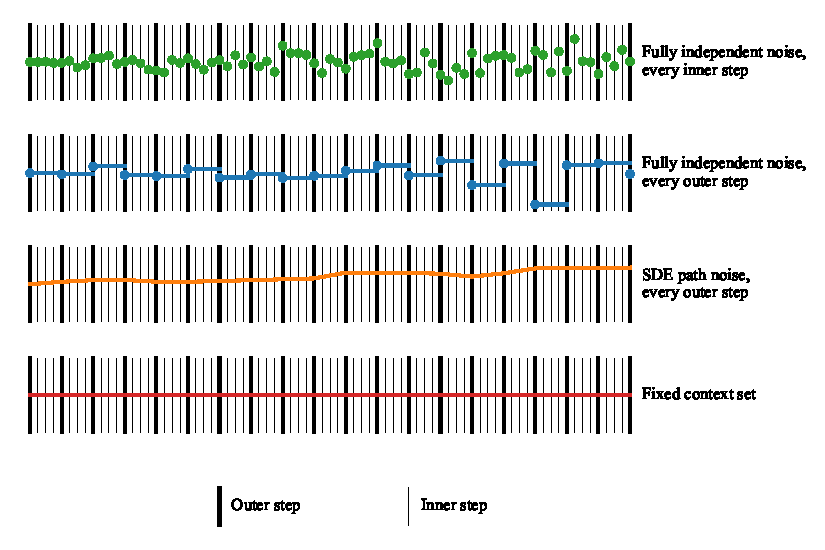
\includegraphics{images/geomndp/compare_noising_schemes.pdf}
	\caption{Comparison of different context noising schemes for the conditional sampling.}
	\label{fig:noise_schemes}
\end{figure}
The main trade-off of different schemes is the speed at which the noise can be sampled vs sample diversity.
In the Euclidean case, we have a closed form for the evolution of the marginal density of the context point under the forward SDE.
In this case sampling the noise at a given time is \(\c{O}(1)\) cost.
On the other hand, in some instances such as nosing stochastic differential equations on general manifolds, we have to simulate this noise by discretising the equation.
In this case, it is \(\c{O}(n)\) cost, where \(n\) is the number of discretisation steps in the stochastic differential equation.
For \(N\) outer steps and \(I\) inner steps, the complexity of the different noising schemes is compared in \cref{tab:noise_comp}.
Note the conditional sampling scheme other than the noise sampling is \(\c{O}(NI)\) complexity.
\begin{table}[h]
	\centering
	\setlength\tabcolsep{0pt}
	\begin{tabular*}{\textwidth}{@{\extracolsep{\fill}}lrr}
		\toprule
		{\scshape Scheme}                              & {\scshape Closed-form noise} & {\scshape Simulated noise} \\
		\midrule
		{\textsc Re-sample noise at every inner step} & \(\c{O}(NI)\)                 & \(\c{O}(N^2I^2)\)           \\
		{\textsc Re-sample noise at every outer step} & \(\c{O}(N)\)                  & \(\c{O}(N^2)\)              \\
		{\textsc Sampling an SDE path on the context} & \(\c{O}(N)\)                  & \(\c{O}(N)\)                \\
		{\textsc No noise applied}                    & -                           & -                         \\
		\bottomrule
	\end{tabular*}
	\caption{Comparison of complexity of different noise sampling schemes for the context set.}
	\label{tab:noise_comp}
\end{table}

\subsection{Likelihood evaluation}

The likelihood ordinary differential equation formulation for computing likelihoods of the marginals in \cref{sec:euclidean_geom_ndp} applies immediately.

For conditional samples using the Langevin sampling method however a similar formulation is not possible.
Instead, we rely on the conditional probability rule to evaluate conditional likelihoods, \(p_{x^o|\v{x}^c}(y^o|\v{y}^c) = p_{x^o,\v{x}^c}(y^o,\v{y}^c) / p_{\v{x}^c}(\v{y}^c)\).
This can be done by solving two probability flow ordinary differential equations on the joint evaluation and context set, and only on the context set.

% \section{Geometric neural diffusion processes} \label{sec:diffusion_sp}

% \subsection{Continuous diffusion on function spaces}
% \label{sec:functional_diffusion}
% We construct a diffusion model on functions \(f: \c{X} \rightarrow \c{Y}\) , with \(\c{Y}=\R^d\), by defining a diffusion model for every finite set of marginals.
% Most prior works on infinite-dimensional diffusions consider a noising process on the space of functions \parencite{kerrigan2022Diffusion,pidstrigach2023InfiniteDimensional,lim2023score}.
% In theory, this allows the model to define a consistent distribution over all the finite marginals of the process being modelled.
% In practice, however, only finite marginals can be modelled on a computer and the score function needs to be approximated, and at this step lose consistency over the marginals.
% The only work to stay fully consistent in implementation is \textcite{phillips2022spectral}, at the cost of limiting functions that can be modelled to a finite-dimensional subspace.
% With this in mind, we eschew the technically laborious process of defining diffusions over the infinite-dimension space and work solely on the finite marginals following \textcite{dutordoir2022Neural}.
% We find that in practice consistency can be well learned from data see \Cref{sec:experiments-gndp}, and this allows for more flexible choices of score network architecture and easier training.

% \textbf{Noising process.}
% We assume we are given a data process \((\v{Y}_0(x))_{x \in \c{X}}\).
% Given any \(x=(x^1, \dots, x^n) \in \c{X}^n\), we consider the following forward \emph{noising} process \((\v{Y}_t(x))_{t \geq 0} \triangleq (\v{Y}_t(x^1),\dots,\v{Y}_t(x^n))_{t \geq 0} = (\v{Y}_t^1,\dots,\v{Y}_t^n)_{t \geq 0} \in \c{Y}^n\) defined by the following multivariate stochastic differential equation \begin{equation}\label{eq:forward_SDE_sp} \end{equation} where \(\mathrm{K}(x,x)_{i,j} = k(x^i, x^j)\) with \(k:\c{X} \times \c{X} \rightarrow \R\) a kernel 

% In the specific instance where \(k(x,x') = \delta_{x}(x')\), then the limiting process \(\v{Y}_\infty\) is simply \emph{white noise}, whilst other choices such as the squared-exponential or Mat\'ern kernel would lead to the associated Gaussian limiting process \(\v{Y}_\infty\).
% Note that the \emph{white noise} setting is not covered by the existing theory of functional diffusion models, as a Hilbert space and a square integral kernel are required, see ~\textcite{kerrigan2022Diffusion} for instance.

% \textbf{Denoising process.}
% Under mild conditions on the distribution of \(\v{Y}_0(x)\), the time-reversal process \((\bar{\v{Y}}_t(x))_{t \geq 0}\) also satisfies an stochastic differential equation~\parencite{cattiaux2021time,haussmann1986time} given by \begin{equation}\label{eq:backward_SDE_dupref2} \textstyle \mathrm{d} \bar{\v{Y}}_t(x) = \{-\tfrac{1}{2} (m(x) - \bar{\v{Y}}_t(x)) + \mathrm{K}(x,x) \nabla \log p_{T-t}(\bar{\v{Y}}_t(x)) \} \beta_{T-t} \mathrm{d} t + \beta_{T-t}^{1/2} \mathrm{K}(x,x)^{1/2} \mathrm{d} \v{B}_t, \end{equation} with \(\bar{\v{Y}}_0 \sim \mathrm{GP} (m, k)\) and \(p_t\) the density of \(\mathbf{Y}_t(x)\) w.r.t.~the Lebesgue measure.
% In practice, the Stein score \(\log p_{T-t}\) is not tractable and must be approximated by a neural network.
% We then consider the generative stochastic process model defined by first sampling \(\bar{\v{Y}}_0 \sim \mathrm{GP} (m, k)\) and then simulating the reverse diffusion \eqref{eq:backward_SDE_dupref2} (e.g.\ via Euler-Maruyama discretisation).

% \textbf{Manifold valued outputs.}
% So far we have defined our generative model with \(\c{Y} = \R^d\), we can readily extend the methodology to manifold-valued functional models using \emph{Riemannian} diffusion models such as \cite{de2022riemannian,huang2022riemannian}, see \cref{sec:manifold_valued}.
% One of the main notable difference is that in the case where \(\c{Y}\) is a \emph{compact} manifold, we replace the Ornstein-Uhlenbeck process by a Brownian motion which targets the uniform distribution.

% \textbf{Training.}
% As the reverse stochastic differential equation \eqref{eq:backward_SDE_dupref2} involves the preconditioned score \(\mathrm{K}(x, x) \nabla \log p_t\), we directly approximate it with a neural network \((\mathrm{Ks})_\theta: [0, T] \times \c{X}^n \times \c{Y}^n \rightarrow T \c{Y}^n\), where \(T \c{Y}\) is the tangent bundle of \(\c{Y}\),see \cref{sec:manifold_valued}.
% The conditional score of the noising process \eqref{eq:forward_SDE_sp} is given by \begin{equation} \textstyle \nabla_{{\v{Y}}_t} \log p_{t}({\v{Y}}_t(x)| \v{Y}_0(x)) = - \Sigma_{t|0}^{-1} (\v{Y}_t(x) - m_{t|0}) = - \sigma_{t|0}^{-1} \mathrm{K}(x,x)^{-1/2} \varepsilon , \end{equation} since \(\v{Y}_t = m_{t|0} + \Sigma_{t|0}^{1/2} \varepsilon\) with \(\varepsilon \sim \mathrm{N}(0, \m{I})\), and \(\Sigma_{t|0} = \sigma_{t|0}^2 \mathrm{K}\) with \(\sigma_{t|0} = (1 - \mathrm{e}^{-\int_{0}^t \beta(s) \mathrm{d} s})^{1/2}\), see \cref{sec:multivariate_ou}.
% We learn the preconditioned score \((\mathrm{Ks})_\theta\) by minimising the following denoising score matching (DSM) loss~\parencite{Vincent2010} weighted by \(\Lambda(t) = \sigma_{t|0}^2~\mathrm{K}^\top \mathrm{K}\) \begin{align} \label{eq:loss} \textstyle \mathcal{L}(\theta; \Lambda(t)) = \mathbb{E} [\| \mathrm{s}_\theta(t, \v{Y}_t) - \nabla \log p_{t}({\v{Y}}_t| \v{Y}_0)\|_{\Lambda(t)}^2 ] = \mathbb{E} [ \| \sigma_{t|0}\cdot (\mathrm{K}s)_\theta(t,\v{Y}_t) + \mathrm{K}^{1/2} \varepsilon \|_2^2 ] , \end{align} where \(\|x\|^2_\Lambda = x^\top \Lambda x\).
% Note that when targeting a unit-variance white noise, then \(\mathrm{K} = \m{I}\) and the loss \eqref{eq:loss} reverts to the DSM loss with weighting \(\lambda(t)=1/\sigma_{t|0}^2\)~\parencite{song2020score}.
% In \cref{sec:multivariate_ou_score}, we explore several preconditioning terms and associated weighting \(\Lambda(t)\).
% Overall, we found the preconditioned score \(\mathrm{K} \nabla \log p_t\) parameterisation, in combination with the \(\ell_2\) loss, to perform best, as shown by the ablation study in \cref{fig:app:score-parametrization-ablation}.

% \subsection{Invariant neural diffusion processes}
% \label{sec:equiv_ndp}

% In this section, we show how we can incorporate geometrical constraints into the functional diffusion model introduced in the previous \cref{sec:functional_diffusion}.
% In particular, given a group \(G\), we aim to build a generative model over steerable tensor fields as defined in \cref{sec:background}.

% \textbf{Invariant process.}
% A stochastic process \(f \sim \mu\) is said to be \(G-\)invariant if \(\mu(g \cdot \mathsf{A}) = \mu(\mathsf{A})\) for any \(g \in G\), with \(\mu \in \mathcal{P}(\c{C}(\c{X}, \c{Y}))\), where \(\mathcal{P}\) is the space of probability measure on the space of continuous functions and \(\mathsf{A} \subset \c{C}(\c{X}, \c{Y})\) measurable.
% From a sample perspective, this means that with input-output pairs \(\mathcal{C} = \{(x^i, y^i)\}_{i=1}^n\), and denoting the action of \(G\) on this set as \(g \cdot \mathcal{C} \triangleq \{(g \cdot x^i, \rho(g) y^i)\}_{i=1}^n\), \(f \sim \mu\) is \(G-\)invariant if and only if \(g \cdot \mathcal{C}\) has the same distribution as \(\mathcal{C}\).
% In what follows, we aim to derive sufficient conditions on the model introduced in \cref{sec:diffusion_sp} so that it satisfies this \(G\)-invariance property.
% First, we recall such a necessary and sufficient condition for Gaussian processes.
% \begin{proposition}{Invariant (stationary) Gaussian process \parencite{holderrieth2021equivariant}.}{}
% 	\label{prop:inv_gp}
% 	We have that a Gaussian process \(\mathrm{GP}(m, k)\) is \(G\)-invariant if and only if its mean \(m\) and covariance \(k\) are suitably \(G\)-equivariant---that is, for all \(x,x' \in \c{X}, g \in G\) \begin{align} m(g \cdot x) = \rho(g) m(x) \ \ \text{and} \ \ k(g \cdot x, g \cdot x') = \rho(g) k(x, x') \rho(g)^\top.
% 	\end{align}
% \end{proposition}
% Trivial examples of \(\groupE{}\)-equivariant kernels include diagonal kernels \(k = k_0 \m{I}\) with \(k_0\) invariant~\parencite{holderrieth2021equivariant}, but see \cref{sec:app_vec_gp} for non trivial instances introduced by \textcite{macedo2010learning}.
% Building on \cref{prop:inv_gp}, we then state that our introduced neural diffusion process 

% \begin{proposition}{Invariant neural diffusion process~\parencite{yim2023se}.
% 	}{}
% 	\label{prop:inv_prior}
% 	We denote by \((\bar{\v{Y}}_t(x))_{t \in [0, T]}\) the process induced by the time-reversal stochastic differential equation \eqref{eq:backward_SDE_dupref2} where the score is approximated by a score network \(\mathbf{s}_\theta: [0, T] \times \c{X}^n \times \c{Y}^n \rightarrow T \c{Y}^n\), and the limiting process is given by \(\mathcal{L}(\bar{\v{Y}}_0) = \mathrm{GP}(m, k)\).
% 	Assuming \(m\) and \(k\) are respectively \(G\)-equivariant per \cref{prop:inv_gp}, if we additionally have that the score network is \(G\)-equivariant vector field, i.e.\ \(\mathbf{s}_\theta(t, g\cdot x, \rho(g) {y}) = \rho(g) \mathbf{s}_\theta(t, x, {y})\) for all \(x \in \c{X}, g \in G\), then for any \({t \in [0, T]}\) the process \((\bar{\v{Y}}_t(x))_{x \in \c{X}}\) is \(G\)-invariant.
% \end{proposition}

% This result can be proved in two ways, from the probability flow ODE perspective or directly in terms of stochastic differential equation via Fokker-Planck, see \cref{sec:proof_inv_prior}.
% In particular, when modelling an invariant scalar data process \(({\v{Y}}_0(x))_{x \in \c{X}}\) such as a temperature field, we need the score network to admits the invariance constraint \(\mathbf{s}_\theta(t, g\cdot x, {y}) = \mathbf{s}_\theta(t, x, {y})\).

% \textbf{Equivariant conditional process.}
% \begin{figure*}[t]
% 	\centering
% 	\begin{subfigure}[t]{0.49\textwidth}
% 		\centering
% 		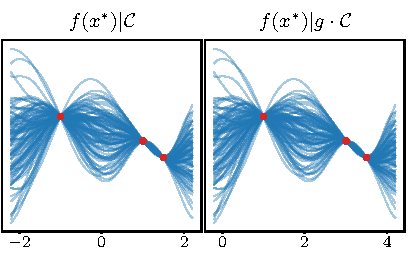
\includegraphics[width=1.\linewidth,trim={0 0 0 0},clip]{images/geomndp/1d/conditional_ndp_shift.pdf}
% 	\end{subfigure}
% 	\begin{subfigure}[t]{0.49\textwidth}
% 		\centering
% 		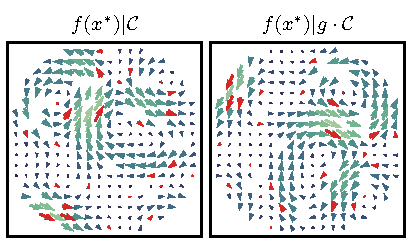
\includegraphics[width=1.\linewidth,trim={0 0 0 0},clip]{images/geomndp/2d/conditional_ndp_rot.pdf}
% 	\end{subfigure}
% 	\caption{
% 		Samples from equivariant neural diffusion processes conditioned on context set \(\mathcal{C}\) (\textcolor{tabred}{in red}) for scalar (\emph{Left}) and 2D vector (\emph{Right}) fields.
% 		Same model is then conditioned on transformed context \(g \cdot \mathcal{C}\), with group element \(g\) being a translation of length \(2\) (\emph{Left}) or a \(90^{\circ}\) rotation (\emph{Right}).
% 	}
% 	\label{fig:posterior_model}
% \end{figure*}
% Often precedence is given to modelling the predictive process given a set of observations \(\mathcal{C} = \{(x^c, y^c)\}_{c \in C}\).
% In this context, the conditional process inherits the symmetry of the prior process in the following sense.
% A stochastic process with distribution \(\mu\) given a context \(\mathcal{C}\) is said to be conditionally \(G-\)equivariant if the conditional satisfies \(\mu(\mathsf{A} | g \cdot \mathcal{C}) = \mu(g \cdot \mathsf{A} |\mathcal{C})\) for any \(g \in G\) and \(\mathsf{A} \in \mathrm{C}(\mathcal{X},\c{Y})\) measurable, as illustrated in \cref{fig:posterior_model}.
% \begin{proposition}{Equivariant conditional process.}{}
% 	\label{prop:equiv_posterior}
% \end{proposition}
% Originally stated in \cite{holderrieth2021equivariant} in the case where the process is over functions of the form \(f: \R^n\to \R^d\) and marginals with density w.r.t.
% \ the Lebesgue measure, we prove \cref{prop:equiv_posterior} for SPs over generic fields on manifolds in terms only of the measure of the process (\cref{sec:equiv_posterior}).

% \subsection{Conditional sampling}
% \label{sec:conditional_sampling}

% \begin{figure}
% 	\centering
% 	\begin{center}
% 		% \resizebox{0.5\linewidth}{!}{
% 			\begin{tikzpicture}
% 				\Large
% 				\draw [stealth-, line width = .05cm] (0,0) .. controls  (2,-4) and (3.,2) .. (6,0);
% 				\draw [-stealth, line width = .05cm, tabblue, dashed] (0,0) -- (1.3,-2.3);
% 				\draw [-stealth, line width = .05cm, tabred, dashed] (1.3,-2.3) -- (1.3,-1.9);
% 				\draw [-stealth, line width = .05cm, tabred, dashed] (1.3,-1.9) -- (1.3,-1.7);
% 				\draw [-stealth, line width = .05cm, tabred, dashed] (1.3,-1.7) -- (1.3,-1.4);
% 				\draw [-stealth, line width = .05cm, tabblue, dashed] (1.3,-1.45) -- (2.8,-1.35);
% 				\draw [-stealth, line width = .05cm, tabred, dashed] (2.8,-1.35) -- (2.4, -0.9);
% 				\node [below=0.2cm] at (6,0) {\(p_0\)};
% 				\node [left=0.0cm] at (0,0) {\(\mathcal{L}(\bar{\v{Y}}_0) = p_T\)};
% 				\node [left=0.2cm] at (1.3,-2.1) {\(\mathcal{L}(\bar{\v{Y}}_\gamma^0)\)};
% 				\node [right=0.1cm] at (1.3,-2.) {\(\mathcal{L}(\bar{\v{Y}}_\gamma^1)\)};
% 				\node [right=0.1cm] at (1.3,-1.65) {\(\cdots\)};
% 				\node [above=0.05cm] at (1.3,-1.35) {\(p_{\gamma}\)};
% 				\node [below right=0.1cm] at (2.8,-0.8) {\(\mathcal{L}(\bar{\v{Y}}_{2\gamma}^0)\)};
% 				\node [right=0.1cm] at (2.6, -0.7) {\(\mathcal{L}(\bar{\v{Y}}_{2\gamma}^1)\)};
% 				\node [above left=0.05cm] at (2.6, -0.9) {\(p_{2\gamma}\)};
% 			\end{tikzpicture}
% 		% }
% 	\end{center}
% 	\caption{
% 		Illustration of Langevin corrected conditional sampling.
% 		The black line represents the noising process dynamics \((p_t)_{t \in \cbr{0,T}}\).
% 		The \textcolor{tabblue}{time reversal (i.e.\ predictor)} step, is combined with a \textcolor{tabred}{Langevin corrector} step projecting back onto the dynamics.
% 	}
% 	\label{fig:predictor_corrector}
% \end{figure}
% There exist several methods to perform conditional sampling in diffusion models such as: replacement sampling, amortisation and conditional guidance.
% Replacement sampling is not exact and do not recover the correct conditional distributions.
% SMC based methods have been proposed to correct this procedure but they suffer from the limitations of SMC and scale poorly with the dimension \parencite{trippe2022Diffusion}.
% On the other hand, amortisation, require the retraining of the score network for each different conditional task which is impractical in our setting where the context length might change.
% Conditional guidance is a popular method in state-of-the-art image diffusion models but does not recover the true posterior distribution.

% Here we propose a new method for sampling from exact conditional distributions of NDPs using only the score network for the joint distribution.
% Using the fact that the conditional score can be written as \(\nabla_x \log p(x|y) = \nabla_x \log p(x, y) - \nabla_x \log p(y) = \nabla_x \log p(x, y)\) we can therefore, for any point in the diffusion time, conditionally sample using Langevin dynamics, following the stochastic differential equation \(\mathrm{d} \v{Y}_s = \tfrac{1}{2} \mathrm{K} \nabla \log p_{T-t}(\v{Y}_s) \mathrm{d} s + \sqrt{\mathrm{K}} \mathrm{d} \v{B}_s\), by only applying the diffusion to the variables of interest and holding the others fixed.
% While we could sample directly at the end time this proves difficult in practice.
% Similar to the motivation of \textcite{song2019generative}, we sample along the reverse diffusion, taking a number of conditional Langevin steps at each time.
% In addition, we apply the forward noising stochastic differential equation to the conditioning points at each step, as this puts the combined context and sampling set in a region that the score function will be well learned in training.
% Our procedure is illustrated in \Cref{alg:conditioning_langevin}.
% In \cref{app:conditional_sampling} we draw links between \textsc{RePaint} of \textcite{lugmayr2022repaint} and our scheme.

% \subsection{Likelihood evaluation}

% Similarly to \textcite{song2020score}, we can derive a deterministic ODE which has the same marginal density as the stochastic differential equation \eqref{eq:forward_SDE_sp}, which is given by the `probability flow' Ordinary Differential Equation (ODE), see \Cref{sec:continuous_process}.
% Once the score network is learnt, we can thus use it in conjunction with an ODE solver to compute the likelihood of the model.
% A perhaps more interesting task is to evaluate the predictive posterior likelihood \(p(y^*|x^*,\{x^i,y^i\}_{i \in C})\) given a context set \(\{x^i,y^i\}_{i \in C}\).
% A simple approach is to simply rely on the conditional probability rule evaluate \(p(y^*|x^*,\{x^i,y^i\}_{i \in C}) = p(y^*,\{y^i\}_{i \in C}|x^*,\{x^i\}_{i \in C}) / p(\{y^i\}_{i \in C}|\{x^i\}_{i \in C})\).
% This can be done by solving two probability flow ODEs on the joint evaluation and context set, and only on the context set.
% As the reverse stochastic differential equation \eqref{eq:backward_SDE_dupref2} involves the preconditioned score \(\mathrm{K}(x, x) \nabla \log p_t\), we directly approximate it with a neural network \((\mathrm{Ks})_\theta: [0, T] \times \c{X}^n \times \c{Y}^n \rightarrow T \c{Y}^n\), where \(T \c{Y}\) is the tangent bundle of \(\c{Y}\),see \cref{sec:manifold_valued}.
% The conditional score of the noising process \eqref{eq:forward_SDE_sp} is given by \begin{equation} \textstyle \nabla_{{\v{Y}}_t} \log p_{t}({\v{Y}}_t(x)| \v{Y}_0(x)) = - \Sigma_{t|0}^{-1} (\v{Y}_t(x) - m_{t|0}) = - \sigma_{t|0}^{-1} \mathrm{K}(x,x)^{-1/2} \varepsilon , \end{equation} since \(\v{Y}_t = m_{t|0} + \Sigma_{t|0}^{1/2} \varepsilon\) with \(\varepsilon \sim \mathrm{N}(0, \m{I})\), and \(\Sigma_{t|0} = \sigma_{t|0}^2 \mathrm{K}\) with \(\sigma_{t|0} = (1 - \mathrm{e}^{-\int_{0}^t \beta(s) \mathrm{d} s})^{1/2}\), see \cref{sec:multivariate_ou}.
% We learn the preconditioned score \((\mathrm{Ks})_\theta\) by minimising the following denoising score matching (DSM) loss~\parencite{Vincent2010} weighted by \(\Lambda(t) = \sigma_{t|0}^2~\mathrm{K}^\top \mathrm{K}\) \begin{align} \label{eq:loss} \textstyle \mathcal{L}(\theta; \Lambda(t)) = \mathbb{E} [\| \mathrm{s}_\theta(t, \v{Y}_t) - \nabla \log p_{t}({\v{Y}}_t| \v{Y}_0)\|_{\Lambda(t)}^2 ] = \mathbb{E} [ \| \sigma_{t|0}\cdot (\mathrm{K}s)_\theta(t,\v{Y}_t) + \mathrm{K}^{1/2} \varepsilon \|_2^2 ] , \end{align} where \(\|x\|^2_\Lambda = x^\top \Lambda x\).
% Note that when targeting a unit-variance white noise, then \(\mathrm{K} = \m{I}\) and the loss \eqref{eq:loss} reverts to the DSM loss with weighting \(\lambda(t)=1/\sigma_{t|0}^2\)~\parencite{song2020score}.
% In \cref{sec:multivariate_ou_score}, we explore several preconditioning terms and associated weighting \(\Lambda(t)\).
% Overall, we found the preconditioned score \(\mathrm{K} \nabla \log p_t\) parameterisation, in combination with the \(\ell_2\) loss, to perform best, as shown by the ablation study in \cref{fig:app:score-parametrization-ablation}.

% \subsection{Invariant neural diffusion processes}
% \label{sec:equiv_ndp}

% In this section, we show how we can incorporate geometrical constraints into the functional diffusion model introduced in the previous \cref{sec:functional_diffusion}.
% In particular, given a group \(G\), we aim to build a generative model over steerable tensor fields as defined in \cref{sec:background}.

% \textbf{Invariant process.}
% A stochastic process \(f \sim \mu\) is said to be \(G-\)invariant if \(\mu(g \cdot \mathsf{A}) = \mu(\mathsf{A})\) for any \(g \in G\), with \(\mu \in \mathcal{P}(\c{C}(\c{X}, \c{Y}))\), where \(\mathcal{P}\) is the space of probability measure on the space of continuous functions and \(\mathsf{A} \subset \c{C}(\c{X}, \c{Y})\) measurable.
% From a sample perspective, this means that with input-output pairs \(\mathcal{C} = \{(x^i, y^i)\}_{i=1}^n\), and denoting the action of \(G\) on this set as \(g \cdot \mathcal{C} \triangleq \{(g \cdot x^i, \rho(g) y^i)\}_{i=1}^n\), \(f \sim \mu\) is \(G-\)invariant if and only if \(g \cdot \mathcal{C}\) has the same distribution as \(\mathcal{C}\).
% In what follows, we aim to derive sufficient conditions on the model introduced in \cref{sec:diffusion_sp} so that it satisfies this \(G\)-invariance property.
% First, we recall such a necessary and sufficient condition for Gaussian processes.
% \begin{proposition}{Invariant (stationary) Gaussian process \parencite{holderrieth2021equivariant}.}{}
% 	\label{prop:inv_gp}
% 	We have that a Gaussian process \(\mathrm{GP}(m, k)\) is \(G\)-invariant if and only if its mean \(m\) and covariance \(k\) are suitably \(G\)-equivariant---that is, for all \(x,x' \in \c{X}, g \in G\) \begin{align} m(g \cdot x) = \rho(g) m(x) \ \ \text{and} \ \ k(g \cdot x, g \cdot x') = \rho(g) k(x, x') \rho(g)^\top.
% 	\end{align}
% \end{proposition}
% Trivial examples of \(\groupE{}\)-equivariant kernels include diagonal kernels \(k = k_0 \m{I}\) with \(k_0\) invariant~\parencite{holderrieth2021equivariant}, but see \cref{sec:app_vec_gp} for non trivial instances introduced by \textcite{macedo2010learning}.
% Building on \cref{prop:inv_gp}, we then state that our introduced neural diffusion process 

% \begin{proposition}{Invariant neural diffusion process~\parencite{yim2023se}.
% 	}{}
% 	\label{prop:inv_prior}
% 	We denote by \((\bar{\v{Y}}_t(x))_{t \in [0, T]}\) the process induced by the time-reversal stochastic differential equation \eqref{eq:backward_SDE_dupref2} where the score is approximated by a score network \(\mathbf{s}_\theta: [0, T] \times \c{X}^n \times \c{Y}^n \rightarrow T \c{Y}^n\), and the limiting process is given by \(\mathcal{L}(\bar{\v{Y}}_0) = \mathrm{GP}(m, k)\).
% 	Assuming \(m\) and \(k\) are respectively \(G\)-equivariant per \cref{prop:inv_gp}, if we additionally have that the score network is \(G\)-equivariant vector field, i.e.\ \(\mathbf{s}_\theta(t, g\cdot x, \rho(g) {y}) = \rho(g) \mathbf{s}_\theta(t, x, {y})\) for all \(x \in \c{X}, g \in G\), then for any \({t \in [0, T]}\) the process \((\bar{\v{Y}}_t(x))_{x \in \c{X}}\) is \(G\)-invariant.
% \end{proposition}

% This result can be proved in two ways, from the probability flow ODE perspective or directly in terms of stochastic differential equation via Fokker-Planck, see \cref{sec:proof_inv_prior}.
% In particular, when modelling an invariant scalar data process \(({\v{Y}}_0(x))_{x \in \c{X}}\) such as a temperature field, we need the score network to admits the invariance constraint \(\mathbf{s}_\theta(t, g\cdot x, {y}) = \mathbf{s}_\theta(t, x, {y})\).

% \textbf{Equivariant conditional process.}
% \begin{figure*}[t]
% 	\centering
% 	\begin{subfigure}[t]{0.49\textwidth}
% 		\centering
% 		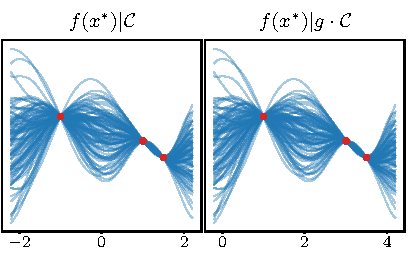
\includegraphics[width=1.\linewidth,trim={0 0 0 0},clip]{images/geomndp/1d/conditional_ndp_shift.pdf}
% 	\end{subfigure}
% 	\begin{subfigure}[t]{0.49\textwidth}
% 		\centering
% 		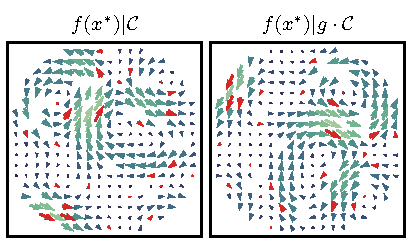
\includegraphics[width=1.\linewidth,trim={0 0 0 0},clip]{images/geomndp/2d/conditional_ndp_rot.pdf}
% 	\end{subfigure}
% 	\caption{
% 		Samples from equivariant neural diffusion processes conditioned on context set \(\mathcal{C}\) (\textcolor{tabred}{in red}) for scalar (\emph{Left}) and 2D vector (\emph{Right}) fields.
% 		Same model is then conditioned on transformed context \(g \cdot \mathcal{C}\), with group element \(g\) being a translation of length \(2\) (\emph{Left}) or a \(90^{\circ}\) rotation (\emph{Right}).
% 	}
% 	\label{fig:posterior_model}
% \end{figure*}
% Often precedence is given to modelling the predictive process given a set of observations \(\mathcal{C} = \{(x^c, y^c)\}_{c \in C}\).
% In this context, the conditional process inherits the symmetry of the prior process in the following sense.
% A stochastic process with distribution \(\mu\) given a context \(\mathcal{C}\) is said to be conditionally \(G-\)equivariant if the conditional satisfies \(\mu(\mathsf{A} | g \cdot \mathcal{C}) = \mu(g \cdot \mathsf{A} |\mathcal{C})\) for any \(g \in G\) and \(\mathsf{A} \in \mathrm{C}(\mathcal{X},\c{Y})\) measurable, as illustrated in \cref{fig:posterior_model}.
% \begin{proposition}{Equivariant conditional process.}{}
% 	\label{prop:equiv_posterior}
% \end{proposition}
% Originally stated in \cite{holderrieth2021equivariant} in the case where the process is over functions of the form \(f: \R^n\to \R^d\) and marginals with density w.r.t.
% \ the Lebesgue measure, we prove \cref{prop:equiv_posterior} for SPs over generic fields on manifolds in terms only of the measure of the process (\cref{sec:equiv_posterior}).

% \subsection{Conditional sampling}
% \label{sec:conditional_sampling}

% \begin{figure}
% 	\centering
% 	\begin{center}
% 		% \resizebox{0.5\linewidth}{!}{
% 			\begin{tikzpicture}
% 				\Large
% 				\draw [stealth-, line width = .05cm] (0,0) .. controls  (2,-4) and (3.,2) .. (6,0);
% 				\draw [-stealth, line width = .05cm, tabblue, dashed] (0,0) -- (1.3,-2.3);
% 				\draw [-stealth, line width = .05cm, tabred, dashed] (1.3,-2.3) -- (1.3,-1.9);
% 				\draw [-stealth, line width = .05cm, tabred, dashed] (1.3,-1.9) -- (1.3,-1.7);
% 				\draw [-stealth, line width = .05cm, tabred, dashed] (1.3,-1.7) -- (1.3,-1.4);
% 				\draw [-stealth, line width = .05cm, tabblue, dashed] (1.3,-1.45) -- (2.8,-1.35);
% 				\draw [-stealth, line width = .05cm, tabred, dashed] (2.8,-1.35) -- (2.4, -0.9);
% 				\node [below=0.2cm] at (6,0) {\(p_0\)};
% 				\node [left=0.0cm] at (0,0) {\(\mathcal{L}(\bar{\v{Y}}_0) = p_T\)};
% 				\node [left=0.2cm] at (1.3,-2.1) {\(\mathcal{L}(\bar{\v{Y}}_\gamma^0)\)};
% 				\node [right=0.1cm] at (1.3,-2.) {\(\mathcal{L}(\bar{\v{Y}}_\gamma^1)\)};
% 				\node [right=0.1cm] at (1.3,-1.65) {\(\cdots\)};
% 				\node [above=0.05cm] at (1.3,-1.35) {\(p_{\gamma}\)};
% 				\node [below right=0.1cm] at (2.8,-0.8) {\(\mathcal{L}(\bar{\v{Y}}_{2\gamma}^0)\)};
% 				\node [right=0.1cm] at (2.6, -0.7) {\(\mathcal{L}(\bar{\v{Y}}_{2\gamma}^1)\)};
% 				\node [above left=0.05cm] at (2.6, -0.9) {\(p_{2\gamma}\)};
% 			\end{tikzpicture}
% 		% }
% 	\end{center}
% 	\caption{
% 		Illustration of Langevin corrected conditional sampling.
% 		The black line represents the noising process dynamics \((p_t)_{t \in \cbr{0,T}}\).
% 		The \textcolor{tabblue}{time reversal (i.e.\ predictor)} step, is combined with a \textcolor{tabred}{Langevin corrector} step projecting back onto the dynamics.
% 	}
% 	\label{fig:predictor_corrector}
% \end{figure}
% There exist several methods to perform conditional sampling in diffusion models such as: replacement sampling, amortisation and conditional guidance.
% Replacement sampling is not exact and do not recover the correct conditional distributions.
% SMC based methods have been proposed to correct this procedure but they suffer from the limitations of SMC and scale poorly with the dimension \parencite{trippe2022Diffusion}.
% On the other hand, amortisation, require the retraining of the score network for each different conditional task which is impractical in our setting where the context length might change.
% Conditional guidance is a popular method in state-of-the-art image diffusion models but does not recover the true posterior distribution.

% Here we propose a new method for sampling from exact conditional distributions of NDPs using only the score network for the joint distribution.
% Using the fact that the conditional score can be written as \(\nabla_x \log p(x|y) = \nabla_x \log p(x, y) - \nabla_x \log p(y) = \nabla_x \log p(x, y)\) we can therefore, for any point in the diffusion time, conditionally sample using Langevin dynamics, following the stochastic differential equation \(\mathrm{d} \v{Y}_s = \tfrac{1}{2} \mathrm{K} \nabla \log p_{T-t}(\v{Y}_s) \mathrm{d} s + \sqrt{\mathrm{K}} \mathrm{d} \v{B}_s\), by only applying the diffusion to the variables of interest and holding the others fixed.
% While we could sample directly at the end time this proves difficult in practice.
% Similar to the motivation of \textcite{song2019generative}, we sample along the reverse diffusion, taking a number of conditional Langevin steps at each time.
% In addition, we apply the forward noising stochastic differential equation to the conditioning points at each step, as this puts the combined context and sampling set in a region that the score function will be well learned in training.
% Our procedure is illustrated in \Cref{alg:conditioning_langevin}.
% In \cref{app:conditional_sampling} we draw links between \textsc{RePaint} of \textcite{lugmayr2022repaint} and our scheme.

% \subsection{Likelihood evaluation}

% Similarly to \textcite{song2020score}, we can derive a deterministic ODE which has the same marginal density as the stochastic differential equation \eqref{eq:forward_SDE_sp}, which is given by the `probability flow' Ordinary Differential Equation (ODE), see \Cref{sec:continuous_process}.
% Once the score network is learnt, we can thus use it in conjunction with an ODE solver to compute the likelihood of the model.
% A perhaps more interesting task is to evaluate the predictive posterior likelihood \(p(y^*|x^*,\{x^i,y^i\}_{i \in C})\) given a context set \(\{x^i,y^i\}_{i \in C}\).
% A simple approach is to simply rely on the conditional probability rule evaluate \(p(y^*|x^*,\{x^i,y^i\}_{i \in C}) = p(y^*,\{y^i\}_{i \in C}|x^*,\{x^i\}_{i \in C}) / p(\{y^i\}_{i \in C}|\{x^i\}_{i \in C})\).
% This can be done by solving two probability flow ODEs on the joint evaluation and context set, and only on the context set.
% As the reverse stochastic differential equation \eqref{eq:backward_SDE_dupref2} involves the preconditioned score \(\mathrm{K}(x, x) \nabla \log p_t\), we directly approximate it with a neural network \((\mathrm{Ks})_\theta: [0, T] \times \c{X}^n \times \c{Y}^n \rightarrow T \c{Y}^n\), where \(T \c{Y}\) is the tangent bundle of \(\c{Y}\),see \cref{sec:manifold_valued}.
% The conditional score of the noising process \eqref{eq:forward_SDE_sp} is given by \begin{equation} \textstyle \nabla_{{\v{Y}}_t} \log p_{t}({\v{Y}}_t(x)| \v{Y}_0(x)) = - \Sigma_{t|0}^{-1} (\v{Y}_t(x) - m_{t|0}) = - \sigma_{t|0}^{-1} \mathrm{K}(x,x)^{-1/2} \varepsilon , \end{equation} since \(\v{Y}_t = m_{t|0} + \Sigma_{t|0}^{1/2} \varepsilon\) with \(\varepsilon \sim \mathrm{N}(0, \m{I})\), and \(\Sigma_{t|0} = \sigma_{t|0}^2 \mathrm{K}\) with \(\sigma_{t|0} = (1 - \mathrm{e}^{-\int_{0}^t \beta(s) \mathrm{d} s})^{1/2}\), see \cref{sec:multivariate_ou}.
% We learn the preconditioned score \((\mathrm{Ks})_\theta\) by minimising the following denoising score matching (DSM) loss~\parencite{Vincent2010} weighted by \(\Lambda(t) = \sigma_{t|0}^2~\mathrm{K}^\top \mathrm{K}\) \begin{align} \label{eq:loss} \textstyle \mathcal{L}(\theta; \Lambda(t)) = \mathbb{E} [\| \mathrm{s}_\theta(t, \v{Y}_t) - \nabla \log p_{t}({\v{Y}}_t| \v{Y}_0)\|_{\Lambda(t)}^2 ] = \mathbb{E} [ \| \sigma_{t|0}\cdot (\mathrm{K}s)_\theta(t,\v{Y}_t) + \mathrm{K}^{1/2} \varepsilon \|_2^2 ] , \end{align} where \(\|x\|^2_\Lambda = x^\top \Lambda x\).
% Note that when targeting a unit-variance white noise, then \(\mathrm{K} = \m{I}\) and the loss \eqref{eq:loss} reverts to the DSM loss with weighting \(\lambda(t)=1/\sigma_{t|0}^2\)~\parencite{song2020score}.
% In \cref{sec:multivariate_ou_score}, we explore several preconditioning terms and associated weighting \(\Lambda(t)\).
% Overall, we found the preconditioned score \(\mathrm{K} \nabla \log p_t\) parameterisation, in combination with the \(\ell_2\) loss, to perform best, as shown by the ablation study in \cref{fig:app:score-parametrization-ablation}.

% \subsection{Invariant neural diffusion processes}
% \label{sec:equiv_ndp}

% In this section, we show how we can incorporate geometrical constraints into the functional diffusion model introduced in the previous \cref{sec:functional_diffusion}.
% In particular, given a group \(G\), we aim to build a generative model over steerable tensor fields as defined in \cref{sec:background}.

% \textbf{Invariant process.}
% A stochastic process \(f \sim \mu\) is said to be \(G-\)invariant if \(\mu(g \cdot \mathsf{A}) = \mu(\mathsf{A})\) for any \(g \in G\), with \(\mu \in \mathcal{P}(\c{C}(\c{X}, \c{Y}))\), where \(\mathcal{P}\) is the space of probability measure on the space of continuous functions and \(\mathsf{A} \subset \c{C}(\c{X}, \c{Y})\) measurable.
% From a sample perspective, this means that with input-output pairs \(\mathcal{C} = \{(x^i, y^i)\}_{i=1}^n\), and denoting the action of \(G\) on this set as \(g \cdot \mathcal{C} \triangleq \{(g \cdot x^i, \rho(g) y^i)\}_{i=1}^n\), \(f \sim \mu\) is \(G-\)invariant if and only if \(g \cdot \mathcal{C}\) has the same distribution as \(\mathcal{C}\).
% In what follows, we aim to derive sufficient conditions on the model introduced in \cref{sec:diffusion_sp} so that it satisfies this \(G\)-invariance property.
% First, we recall such a necessary and sufficient condition for Gaussian processes.
% \begin{proposition}{Invariant (stationary) Gaussian process \parencite{holderrieth2021equivariant}.}{}
% 	\label{prop:inv_gp}
% 	We have that a Gaussian process \(\mathrm{GP}(m, k)\) is \(G\)-invariant if and only if its mean \(m\) and covariance \(k\) are suitably \(G\)-equivariant---that is, for all \(x,x' \in \c{X}, g \in G\) \begin{align} m(g \cdot x) = \rho(g) m(x) \ \ \text{and} \ \ k(g \cdot x, g \cdot x') = \rho(g) k(x, x') \rho(g)^\top.
% 	\end{align}
% \end{proposition}
% Trivial examples of \(\groupE{}\)-equivariant kernels include diagonal kernels \(k = k_0 \m{I}\) with \(k_0\) invariant~\parencite{holderrieth2021equivariant}, but see \cref{sec:app_vec_gp} for non trivial instances introduced by \textcite{macedo2010learning}.
% Building on \cref{prop:inv_gp}, we then state that our introduced neural diffusion process 

% \begin{proposition}{Invariant neural diffusion process~\parencite{yim2023se}.
% 	}{}
% 	\label{prop:inv_prior}
% 	We denote by \((\bar{\v{Y}}_t(x))_{t \in [0, T]}\) the process induced by the time-reversal stochastic differential equation \eqref{eq:backward_SDE_dupref2} where the score is approximated by a score network \(\mathbf{s}_\theta: [0, T] \times \c{X}^n \times \c{Y}^n \rightarrow T \c{Y}^n\), and the limiting process is given by \(\mathcal{L}(\bar{\v{Y}}_0) = \mathrm{GP}(m, k)\).
% 	Assuming \(m\) and \(k\) are respectively \(G\)-equivariant per \cref{prop:inv_gp}, if we additionally have that the score network is \(G\)-equivariant vector field, i.e.\ \(\mathbf{s}_\theta(t, g\cdot x, \rho(g) {y}) = \rho(g) \mathbf{s}_\theta(t, x, {y})\) for all \(x \in \c{X}, g \in G\), then for any \({t \in [0, T]}\) the process \((\bar{\v{Y}}_t(x))_{x \in \c{X}}\) is \(G\)-invariant.
% \end{proposition}

% This result can be proved in two ways, from the probability flow ODE perspective or directly in terms of stochastic differential equation via Fokker-Planck, see \cref{sec:proof_inv_prior}.
% In particular, when modelling an invariant scalar data process \(({\v{Y}}_0(x))_{x \in \c{X}}\) such as a temperature field, we need the score network to admits the invariance constraint \(\mathbf{s}_\theta(t, g\cdot x, {y}) = \mathbf{s}_\theta(t, x, {y})\).

% \textbf{Equivariant conditional process.}
% \begin{figure*}[t]
% 	\centering
% 	\begin{subfigure}[t]{0.49\textwidth}
% 		\centering
% 		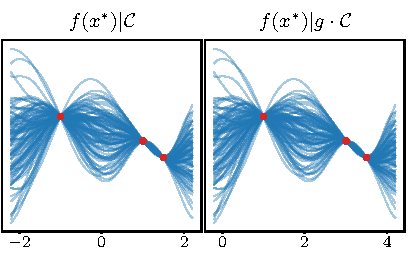
\includegraphics[width=1.\linewidth,trim={0 0 0 0},clip]{images/geomndp/1d/conditional_ndp_shift.pdf}
% 	\end{subfigure}
% 	\begin{subfigure}[t]{0.49\textwidth}
% 		\centering
% 		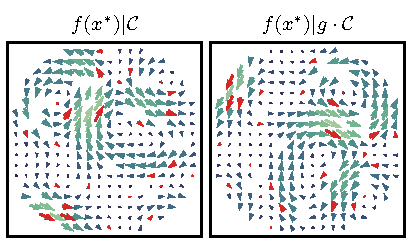
\includegraphics[width=1.\linewidth,trim={0 0 0 0},clip]{images/geomndp/2d/conditional_ndp_rot.pdf}
% 	\end{subfigure}
% 	\caption{
% 		Samples from equivariant neural diffusion processes conditioned on context set \(\mathcal{C}\) (\textcolor{tabred}{in red}) for scalar (\emph{Left}) and 2D vector (\emph{Right}) fields.
% 		Same model is then conditioned on transformed context \(g \cdot \mathcal{C}\), with group element \(g\) being a translation of length \(2\) (\emph{Left}) or a \(90^{\circ}\) rotation (\emph{Right}).
% 	}
% 	\label{fig:posterior_model}
% \end{figure*}
% Often precedence is given to modelling the predictive process given a set of observations \(\mathcal{C} = \{(x^c, y^c)\}_{c \in C}\).
% In this context, the conditional process inherits the symmetry of the prior process in the following sense.
% A stochastic process with distribution \(\mu\) given a context \(\mathcal{C}\) is said to be conditionally \(G-\)equivariant if the conditional satisfies \(\mu(\mathsf{A} | g \cdot \mathcal{C}) = \mu(g \cdot \mathsf{A} |\mathcal{C})\) for any \(g \in G\) and \(\mathsf{A} \in \mathrm{C}(\mathcal{X},\c{Y})\) measurable, as illustrated in \cref{fig:posterior_model}.
% \begin{proposition}{Equivariant conditional process.}{}
% 	\label{prop:equiv_posterior}
% \end{proposition}
% Originally stated in \cite{holderrieth2021equivariant} in the case where the process is over functions of the form \(f: \R^n\to \R^d\) and marginals with density w.r.t.
% \ the Lebesgue measure, we prove \cref{prop:equiv_posterior} for SPs over generic fields on manifolds in terms only of the measure of the process (\cref{sec:equiv_posterior}).

% \subsection{Conditional sampling}
% \label{sec:conditional_sampling}

% \begin{figure}
% 	\centering
% 	\begin{center}
% 		% \resizebox{0.5\linewidth}{!}{
% 			\begin{tikzpicture}
% 				\Large
% 				\draw [stealth-, line width = .05cm] (0,0) .. controls  (2,-4) and (3.,2) .. (6,0);
% 				\draw [-stealth, line width = .05cm, tabblue, dashed] (0,0) -- (1.3,-2.3);
% 				\draw [-stealth, line width = .05cm, tabred, dashed] (1.3,-2.3) -- (1.3,-1.9);
% 				\draw [-stealth, line width = .05cm, tabred, dashed] (1.3,-1.9) -- (1.3,-1.7);
% 				\draw [-stealth, line width = .05cm, tabred, dashed] (1.3,-1.7) -- (1.3,-1.4);
% 				\draw [-stealth, line width = .05cm, tabblue, dashed] (1.3,-1.45) -- (2.8,-1.35);
% 				\draw [-stealth, line width = .05cm, tabred, dashed] (2.8,-1.35) -- (2.4, -0.9);
% 				\node [below=0.2cm] at (6,0) {\(p_0\)};
% 				\node [left=0.0cm] at (0,0) {\(\mathcal{L}(\bar{\v{Y}}_0) = p_T\)};
% 				\node [left=0.2cm] at (1.3,-2.1) {\(\mathcal{L}(\bar{\v{Y}}_\gamma^0)\)};
% 				\node [right=0.1cm] at (1.3,-2.) {\(\mathcal{L}(\bar{\v{Y}}_\gamma^1)\)};
% 				\node [right=0.1cm] at (1.3,-1.65) {\(\cdots\)};
% 				\node [above=0.05cm] at (1.3,-1.35) {\(p_{\gamma}\)};
% 				\node [below right=0.1cm] at (2.8,-0.8) {\(\mathcal{L}(\bar{\v{Y}}_{2\gamma}^0)\)};
% 				\node [right=0.1cm] at (2.6, -0.7) {\(\mathcal{L}(\bar{\v{Y}}_{2\gamma}^1)\)};
% 				\node [above left=0.05cm] at (2.6, -0.9) {\(p_{2\gamma}\)};
% 			\end{tikzpicture}
% 		% }
% 	\end{center}
% 	\caption{
% 		Illustration of Langevin corrected conditional sampling.
% 		The black line represents the noising process dynamics \((p_t)_{t \in \cbr{0,T}}\).
% 		The \textcolor{tabblue}{time reversal (i.e.\ predictor)} step, is combined with a \textcolor{tabred}{Langevin corrector} step projecting back onto the dynamics.
% 	}
% 	\label{fig:predictor_corrector}
% \end{figure}
% There exist several methods to perform conditional sampling in diffusion models such as: replacement sampling, amortisation and conditional guidance.
% Replacement sampling is not exact and do not recover the correct conditional distributions.
% SMC based methods have been proposed to correct this procedure but they suffer from the limitations of SMC and scale poorly with the dimension \parencite{trippe2022Diffusion}.
% On the other hand, amortisation, require the retraining of the score network for each different conditional task which is impractical in our setting where the context length might change.
% Conditional guidance is a popular method in state-of-the-art image diffusion models but does not recover the true posterior distribution.

% Here we propose a new method for sampling from exact conditional distributions of NDPs using only the score network for the joint distribution.
% Using the fact that the conditional score can be written as \(\nabla_x \log p(x|y) = \nabla_x \log p(x, y) - \nabla_x \log p(y) = \nabla_x \log p(x, y)\) we can therefore, for any point in the diffusion time, conditionally sample using Langevin dynamics, following the stochastic differential equation \(\mathrm{d} \v{Y}_s = \tfrac{1}{2} \mathrm{K} \nabla \log p_{T-t}(\v{Y}_s) \mathrm{d} s + \sqrt{\mathrm{K}} \mathrm{d} \v{B}_s\), by only applying the diffusion to the variables of interest and holding the others fixed.
% While we could sample directly at the end time this proves difficult in practice.
% Similar to the motivation of \textcite{song2019generative}, we sample along the reverse diffusion, taking a number of conditional Langevin steps at each time.
% In addition, we apply the forward noising stochastic differential equation to the conditioning points at each step, as this puts the combined context and sampling set in a region that the score function will be well learned in training.
% Our procedure is illustrated in \Cref{alg:conditioning_langevin}.
% In \cref{app:conditional_sampling} we draw links between \textsc{RePaint} of \textcite{lugmayr2022repaint} and our scheme.

% \subsection{Likelihood evaluation}

% Similarly to \textcite{song2020score}, we can derive a deterministic ODE which has the same marginal density as the stochastic differential equation \eqref{eq:forward_SDE_sp}, which is given by the `probability flow' Ordinary Differential Equation (ODE), see \Cref{sec:continuous_process}.
% Once the score network is learnt, we can thus use it in conjunction with an ODE solver to compute the likelihood of the model.
% A perhaps more interesting task is to evaluate the predictive posterior likelihood \(p(y^*|x^*,\{x^i,y^i\}_{i \in C})\) given a context set \(\{x^i,y^i\}_{i \in C}\).
% A simple approach is to simply rely on the conditional probability rule evaluate \(p(y^*|x^*,\{x^i,y^i\}_{i \in C}) = p(y^*,\{y^i\}_{i \in C}|x^*,\{x^i\}_{i \in C}) / p(\{y^i\}_{i \in C}|\{x^i\}_{i \in C})\).
% This can be done by solving two probability flow ODEs on the joint evaluation and context set, and only on the context set.

\section{Related work}

\textbf{Gaussian processes and the neural processes family.}
One important and powerful framework to construct distributions over functional spaces are Gaussian processes \parencite{rasmussen2003gaussian}.
Yet, they are restricted in their modelling capacity and when using exact inference they scale poorly with the number of datapoints.
Recently introduced autoregressive NPs \parencite{bruinsma2023Autoregressive} alleviate this limitation, but they are disadvantaged by the fact that variables early in the auto-regressive generation only have simple distributions (typically Gaussian).
Finally, \cite{dupont2022data} model weights of implicit neural representation using diffusion models.

\paragraph{Stationary stochastic processes.}
The most popular Gaussian process kernels (e.g.\ squared exponential, Mat\'ern) are stationary, that is, they are translation invariant.
This idea can be extended to the entire isometry group of Euclidean spaces \parencite{holderrieth2021equivariant}, allowing for modelling higher order tensor fields, such as wind fields or incompressible fluid velocity \parencite{macedo2010learning}.
Later, \textcite{azangulov2023stationary, azangulov2023stationary2} extended stationary kernels and Gaussian processes to a large class of non-Euclidean spaces, in particular all compact spaces, and symmetric non-compact spaces.
In the context of neural processes, \cite{gordon2019Convolutional} introduced \textsc{ConvCNP} to encode translation equivariance into the predictive process.
They do so by embedding the context into a translation equivariant functional representation which is then decoded with a convolutional neural network.
\textcite{holderrieth2021equivariant} later extended this idea to construct neural processes that are additionally equivariant w.r.t.\ rotations or subgroup thereof.

\paragraph{Spatial structure in diffusion models.}
A variety of approaches have also been proposed to incorporate spatial correlation in the noising process of finite-dimensional diffusion models leveraging the multiscale structure of data \parencite{jing2022subspace,guth2022wavelet,ho2022cascaded,saharia2021image,hoogeboom2022blurring,rissanen2022Generative}.
Our methodology can also be seen as a principled way to modify the forward dynamics in classical denoising diffusion models.
Hence, our contribution can be understood in the light of recent advances in generative modelling on soft and cold denoising diffusion models \parencite{daras2022soft,bansal2022cold,hoogeboom2022blurring}.
Several recent work explicitly introduced a covariance matrix in the Gaussian noise, either on a choice of kernel \parencite{bilos2022Modeling}, based on Discrete Fourier Transform of images \parencite{voleti2022Scorebased}, or via empirical second order statistics (squared pairwise distances and the squared radius of gyration) for protein modelling \parencite{ingrahamIlluminating}.
Alternatively, \parencite{guth2022wavelet} introduced correlation on images leveraging a wavelet basis.

\paragraph{Functional diffusion models.}
Infinite dimensional diffusion models have been investigated in the Euclidean setting in \textcite{kerrigan2022Diffusion,pidstrigach2023InfiniteDimensional,lim2023score,bond2023infty,hagemann2023multilevel,franzese2023continuous,dutordoir2022Neural,phillips2022spectral}.
Most of these works are based on an extension of the diffusion models techniques \textcite{song2020score,ho2020denoising} to the infinite-dimensional space, leveraging tools from the Cameron-Martin theory such as the Feldman-H\'{a}jek theorem \cite{kerrigan2022Diffusion,pidstrigach2023InfiniteDimensional} to define infinite-dimensional Gaussian measures and how they interact.
We refer to \textcite{da2014stochastic} for a thorough introduction to Stochastic Differential Equations in infinite dimension.
\textcite{phillips2022spectral}
consider another approach by defining countable diffusion processes in a
basis.
All these approaches amount to learn a diffusion model with spatial structure.
Note that this induced correlation is necessary for the theory of infinite dimensional stochastic differential equation \parencite{da2014stochastic} to be applied but is not necessary to implement diffusion models \parencite{dutordoir2022Neural}.
Several approaches have been considered for conditional sampling.
\textcite{pidstrigach2023InfiniteDimensional,bond2023infty} modify the reverse diffusion to introduce a guidance term, while
\textcite{dutordoir2022Neural,kerrigan2022Diffusion} use the replacement
method.
Finally, \textcite{phillips2022spectral} amortise the score function w.r.t.
\ the conditioning context.

\section{Experimental results} \label{sec:experiments-gndp}
Our implementation is built on \(\texttt{jax}\)~\cite{jax2018github}, and is publicly available at \url{https://github.com/cambridge-mlg/neural_diffusion_processes}.
Additional details for each experiment can be found in \cref{app:experimental_details}
.
\subsection{1D regression over stationary scalar fields}
\label{sec:1d_regression}
\begin{figure*}
	\centering
	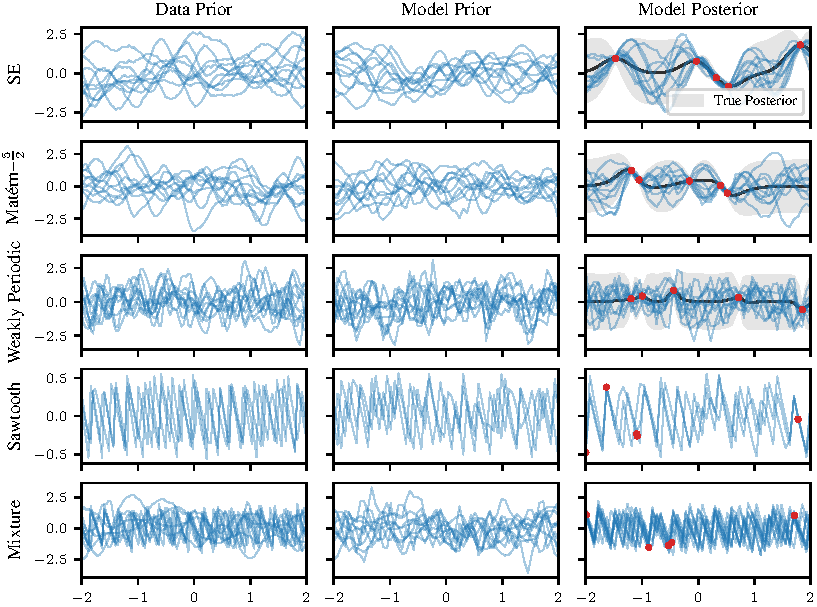
\includegraphics{images/geomndp/1d/plot_regression1d_appendix.pdf}
	\caption{
		Prior and posterior samples (\textcolor{tabblue}{in blue}) from the data process and the GeomNDP  model, with context points \textcolor{tabred}{in red} and posterior mean in {black}.
	}
	\label{fig:1d_regression}
\end{figure*}

% \begin{figure*}[t]
% 	\centering
% 	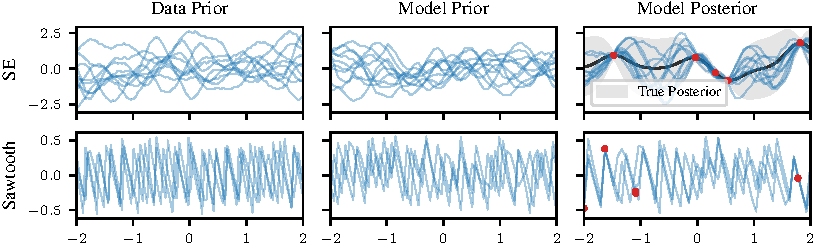
\includegraphics{images/geomndp/1d/plot_regression1d_body.pdf}
% 	% \caption{
% 	% 	Prior and posterior samples (\textcolor{tabblue}{in blue}) from the data process and the GeomNDP  model, with context points \textcolor{tabred}{in red} and posterior mean in {black}.
% 	% }
% 	\label{fig:1d_regression}
% \end{figure*}
We evaluate {\scshape GeomNDPs} on several synthetic 1D regression datasets.
We follow the same experimental setup as \textcite{bruinsma2020Gaussian} which we detail in \cref{app:experimental_details_1d_regression}.
In short, it contains Gaussian (Squared Exponential ({\scshape SE}), {\scshape Mat\'ern\((\tfrac52)\)}, {\scshape Weakly Periodic}) and non-Gaussian ({\scshape Sawtooth} and {\scshape Mixture}) sample paths, where {\scshape Mixture} is a combination of the other four datasets with equal weight.
\Cref{fig:1d_regression} shows samples for each of these datasets.
The Gaussian datasets are corrupted with observation noise with variance \(\sigma^2=0.05^2\).
\Cref{tab:1d_regression} reports the average log-likelihood \(p(y^* | x^*, \c{C})\) across \(4096\) test samples, where the context set size is uniformly sampled between \(1\) and \(10\) and the target has fixed size of \(50\).
All inputs \(x^c, x^*\) are chosen uniformly within their input domain which is \([\text{-}2, 2]\) for the training data and {`interpolation'} evaluation and \([2, 6]\) for the {`generalisation'} evaluation.


\begin{table*}[t]
	% \small
	\centering
	\caption{
		Mean test log-likelihood (TLL) (\(\uparrow\)) \(\pm\) 1 standard error estimated over 4096 test samples are reported.
		Statistically significant best non-GP model is in \textbf{bold}.
		`*' stands for a TLL below \(-10\).
		NP baselines from \textcite{bruinsma2020Gaussian}.
	}
	\label{tab:1d_regression}
	\setlength{\tabcolsep}{3.5pt}
	\begin{tabular}{llrrrrr}
		\toprule
		 &                                                         & \multicolumn{1}{c}{\scshape SE}                                               & \multicolumn{1}{c}{\scshape Mat\'ern-\(\tfrac52\)}                             & \multicolumn{1}{c}{\scshape Weakly Per.}                           & \multicolumn{1}{c}{\scshape Sawtooth}                                         & \multicolumn{1}{c}{\scshape Mixture}                                          \\

		\midrule
		\parbox[t]{2mm}{\multirow{5}{*}{\rotatebox[origin=c]{90}{\textsc{\scalefont{.85}
						Interpolate}.
				}}}
		 & \scshape GP (optimum)                                   & \(\hphantom{-}0.70 { \pm \scriptstyle 0.00 }\)                                  & \(\hphantom{-}0.31 { \pm \scriptstyle 0.00 }\)                                  & \(-0.32 { \pm \scriptstyle 0.00 }\)                                  & -                                                                             & -                                                                             \\
		 & \cellcolor{pearDark!20}\scshape \(\groupT[1]{}-\)GeomNDP & \cellcolor{pearDark!20} \(\hphantom{-}\mathbf{0.72} { \pm \scriptstyle 0.03 }\) & \cellcolor{pearDark!20} \(\hphantom{-}\mathbf{0.32} { \pm \scriptstyle 0.03 }\) & \cellcolor{pearDark!20} \(\mathbf{-0.38} { \pm \scriptstyle 0.03 }\) & \cellcolor{pearDark!20} \(\hphantom{-}\mathbf{3.39} { \pm \scriptstyle 0.04 }\) & \cellcolor{pearDark!20} \(\hphantom{-}\mathbf{0.64} { \pm \scriptstyle 0.08 }\) \\
		 & \scshape NDP\textsuperscript{*}                         & \(\hphantom{-}\mathbf{0.71} { \pm \scriptstyle 0.03 }\)                         & \(\hphantom{-}\mathbf{0.30} { \pm \scriptstyle 0.03 }\)                         & \(\mathbf{-0.37} { \pm \scriptstyle 0.03 }\)                         & \(\hphantom{-}\mathbf{3.39} { \pm \scriptstyle 0.04 }\)                         & \(\hphantom{-}\mathbf{0.64} { \pm \scriptstyle 0.08 }\)                         \\
		 & \scshape GNP                                            & \(\hphantom{-}\mathbf{0.70} { \pm \scriptstyle 0.01 }\)                         & \(\hphantom{-}\mathbf{0.30} { \pm \scriptstyle 0.01 }\)                         & \(-0.47 { \pm \scriptstyle 0.01 }\)                                  & \(\hphantom{-}0.42 { \pm \scriptstyle 0.01 }\)                                  & \(\hphantom{-}0.10 { \pm \scriptstyle 0.02 }\)                                  \\
		 & \scshape ConvNP                                         & \(-0.46 { \pm \scriptstyle 0.01 }\)                                             & \(-0.67 { \pm \scriptstyle 0.01 }\)                                             & \(-1.02 { \pm \scriptstyle 0.01 }\)                                  & \(\hphantom{-}1.20 { \pm \scriptstyle 0.01 }\)                                  & \(-0.50 { \pm \scriptstyle 0.02 }\)                                             \\

		\midrule
		\parbox[t]{2mm}{\multirow{5}{*}{\rotatebox[origin=c]{90}{\textsc  {\scalefont{.85}
						Generalisat}.
				}}}
		 & \scshape GP (optimum)                                   & \(\hphantom{-}0.70 { \pm \scriptstyle 0.00 }\)                                  & \(\hphantom{-}0.31 { \pm \scriptstyle 0.00 }\)                                  & \(-0.32 { \pm \scriptstyle 0.00 }\)                                  & -                                                                             & -                                                                             \\
		 & \cellcolor{pearDark!20}\scshape\(\groupT[1]{}-\)GeomNDP  & \cellcolor{pearDark!20} \(\hphantom{-}\mathbf{0.70} { \pm \scriptstyle 0.02 }\) & \cellcolor{pearDark!20} \(\hphantom{-}\mathbf{0.31} { \pm \scriptstyle 0.02 }\) & \cellcolor{pearDark!20} \(\mathbf{-0.38} { \pm \scriptstyle 0.03 }\) & \cellcolor{pearDark!20} \(\hphantom{-}\mathbf{3.39} { \pm \scriptstyle 0.03 }\) & \cellcolor{pearDark!20} \(\hphantom{-}\mathbf{0.62} { \pm \scriptstyle 0.02 }\) \\
		 & \scshape NDP\textsuperscript{*}                         & *                                                                             & *                                                                             & *                                                                  & *                                                                             & *                                                                             \\
		 & \scshape GNP                                            & \(\hphantom{-}\mathbf{0.69} { \pm \scriptstyle 0.01 }\)                         & \(\hphantom{-}\mathbf{0.30} { \pm \scriptstyle 0.01 }\)                         & \(-0.47 { \pm \scriptstyle 0.01 }\)                                  & \(\hphantom{-}0.42 { \pm \scriptstyle 0.01 }\)                                  & \(\hphantom{-}0.10 { \pm \scriptstyle 0.02 }\)                                  \\
		 & \scshape ConvNP                                         & \(-0.46 { \pm \scriptstyle 0.01 }\)                                             & \(-0.67 { \pm \scriptstyle 0.01 }\)                                             & \(-1.02 { \pm \scriptstyle 0.01 }\)                                  & \(\hphantom{-}1.19 { \pm \scriptstyle 0.01 }\)                                  & \(-0.53 { \pm \scriptstyle 0.02 }\)                                             \\

		\bottomrule
	\end{tabular}
\end{table*}

We compare the performance of GeomNDP to a GP with the true hyperparameters (when available), a (convolutional) Gaussian NP \parencite{bruinsma2020Gaussian}, a convolutional NP \parencite{gordon2019Convolutional} and a vanilla attention-based NDP \parencite{dutordoir2022Neural} which we reformulated in the continuous diffusion process framework to allow for log-likelihood evaluations and thus a fair comparison---denoted NDP\textsuperscript{*}.
We enforce translation invariance in the score network for GeomNDP by subtracting the centre of mass from the input \(x\), inducing stationary scalar fields.

On the GP datasets, {\scshape GNP}, {\scshape ConvNPs} and GeomNDP methods are able to fit the conditionals perfectly---matching the log-likelihood of the GP model.
	{\scshape GNP}'s performance degrades on the non-Gaussian datasets as it is restricted by its conditional Gaussian assumption, whilst {\scshape NDPs} methods still performs well as illustrated on \cref{fig:1d_regression}.
In the bottom rows of \cref{tab:1d_regression}, we assess the models ability to generalise outside of the training input range \(x \in [\text{-}2, 2]\), and evaluate them on a translated grid where context and target points are sampled from \([2,6]\).
Only convolutional NPs ({\scshape GNP} and {\scshape ConvNP}) and {\scshape \(\groupT{1}-\)GeomNDP } are able to model stationary processes and therefore to perform as well as in the interpolation task.
The {\scshape NDP\textsuperscript{*}}, on the contrary, drastically fails at this task.


\textbf{Non white kernels for limiting process.}
The NDP methods in the above experiment target the white kernel \(\mathbbm{1}(x = x')\) in the limiting process.
In \cref{fig:app:score-parametrization-ablation}, we explore different choices for the limiting kernel, such as SE and periodic kernels with short and long lengthscales, along with several score parameterisations, see \cref{sec:app_parameterisation} for a description of these.
We observe that although choosing such kernels gives a head start to the training, it eventually yeilds slightly worse performance.
We attribute this to the additional complexity of learning a non-diagonal covariance.
Finally, across all datasets and limiting kernels, we found the preconditioned score \(\mathrm{K}\nabla \log p_t\) to result in the best performance.

\textbf{Conditional sampling ablation.}
We employ the SE dataset to investigate various configurations of the conditional sampler as we have access to the ground truth conditional distribution through the GP posterior.
In \cref{fig:app:conditional-ablation} we compute the Kullback-Leibler divergence between the samples generated by {\scshape GeomNDP } and the actual conditional distribution across different conditional sampling settings.
Our results demonstrate the importance of performing multiple Langevin dynamics steps during the conditional sampling process.
Additionally, we observe that the choice of noising scheme for the context values \(y_c\) has relatively less impact on the overall outcome.

\subsection{Regression over Gaussian process vector fields}
\label{sec:vec_gp}
% \begin{figure*}[b!]
% 	\centering
% 	% \small
% 	\begin{subfigure}{.49\textwidth}
% 		\setlength{\tabcolsep}{2pt}
% 		\begin{tabular}{lccc}
% 			\toprule
% 			\textsc{Model}                                         & \scshape SE            & \scshape Curl-free     & \scshape Div-free      \\
% 			\midrule
% 			\scshape GP                                            & \({0.56_{\pm 0.00}}\)    & \({0.66_{\pm 0.00}}\)    & \({0.66_{\pm 0.00}}\)    \\
% 			\scshape NDP\textsuperscript{*}                        & \({0.55_{\pm 0.00}}\)    & \({0.62_{\pm 0.01}}\)    & \({0.62_{\pm 0.01}}\)    \\
% 			\rowcolor{pearDark!20} \(\groupE[2]{}\)\scshape-GeomNDP & \(\bm{0.56_{\pm 0.01}}\) & \(\bm{0.65_{\pm 0.01}}\) & \(\bm{0.66_{\pm 0.01}}\) \\
% 			\midrule
% 			\scshape GP (diag.)                                    & \({-1.56_{\pm 0.00}}\)   & \({-1.47_{\pm 0.00}}\)   & \({-1.47_{\pm 0.00}}\)   \\
% 			\(\groupT[2]{}\)\scshape-ConvCNP                        & \({-1.71_{\pm 0.01}}\)   & \({-1.77_{\pm 0.01}}\)   & \({-1.76_{\pm 0.00}}\)   \\
% 			\(\groupE[2]{}\)\scshape-SteerCNP                       & \({-1.61_{\pm 0.00}}\)   & \({-1.57_{\pm 0.00}}\)   & \({-1.57_{\pm 0.01}}\)   \\
% 			\bottomrule
% 		\end{tabular}
% 	\end{subfigure}
% 	\hfill
% 	\begin{subfigure}{.49\textwidth}
% 		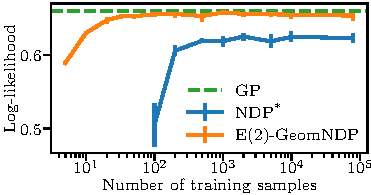
\includegraphics{images/geomndp/2d/ablation_training_samples.pdf}
% 	\end{subfigure}
% 	\caption{
% 		Quantitative results for experiments on GP vector fields.
% 		Mean predictive log-likelihood (\(\uparrow\)) and confidence interval estimated over 5 random seeds.
% 		\emph{Left}: Comparison with neural processes.
% 		Statistically significant results are in \textbf{bold}. \emph{Right:} Ablation study when varying the number of training data samples.
% 	}
% 	\label{fig:vec_gp_results}
% \end{figure*}

\begin{table}
	\setlength{\tabcolsep}{2pt}
	\begin{tabular}{lccc}
		\toprule
		\textsc{Model}                                         & \scshape SE            & \scshape Curl-free     & \scshape Div-free      \\
		\midrule
		\scshape GP                                            & \({0.56_{\pm 0.00}}\)    & \({0.66_{\pm 0.00}}\)    & \({0.66_{\pm 0.00}}\)    \\
		\scshape NDP\textsuperscript{*}                        & \({0.55_{\pm 0.00}}\)    & \({0.62_{\pm 0.01}}\)    & \({0.62_{\pm 0.01}}\)    \\
		\rowcolor{pearDark!20} \(\groupE[2]{}\)\scshape-GeomNDP & \(\bm{0.56_{\pm 0.01}}\) & \(\bm{0.65_{\pm 0.01}}\) & \(\bm{0.66_{\pm 0.01}}\) \\
		\midrule
		\scshape GP (diag.)                                    & \({-1.56_{\pm 0.00}}\)   & \({-1.47_{\pm 0.00}}\)   & \({-1.47_{\pm 0.00}}\)   \\
		\(\groupT[2]{}\)\scshape-ConvCNP                        & \({-1.71_{\pm 0.01}}\)   & \({-1.77_{\pm 0.01}}\)   & \({-1.76_{\pm 0.00}}\)   \\
		\(\groupE[2]{}\)\scshape-SteerCNP                       & \({-1.61_{\pm 0.00}}\)   & \({-1.57_{\pm 0.00}}\)   & \({-1.57_{\pm 0.01}}\)   \\
		\bottomrule
	\end{tabular}
	\caption{
		Quantitative results comparing fitting neural diffusion process models and regular neural process models to samples from GP vector fields.
		Mean predictive log-likelihood (\(\uparrow\)) and confidence interval estimated over 5 random seeds.}
	\label{fig:vec_gp_results_normal}
\end{table}
\begin{figure}
	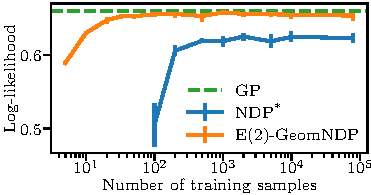
\includegraphics[width=.6\textwidth]{images/geomndp/2d/ablation_training_samples.pdf}
	\caption{
	Quantitative results for an ablation study fitting models to samples from GP vector fields with varying numbers of training data samples.
	Mean predictive log-likelihood (\(\uparrow\)) and confidence interval estimated over 5 random seeds.}
	\label{fig:vec_gp_results_ablation}
\end{figure}



We now focus our attention to modelling equivariant vector fields.
For this, we create datasets using samples from a two-dimensional zero-mean GP with one of the following \(\groupSE{2}\)-equivariant kernels: a diagonal Squared-Exponential ({\scshape SE}) kernel, a zero curl ({\scshape Curl-free}) kernel and a zero divergence ({\scshape Div-free}) kernel, as described in \cref{sec:en_equiv_kernels}.

We equip our model, GeomNDP \!\!\!, with a \(\groupE{2}\)-equivariant score architecture, based on steerable CNNs~\parencite{thomas2018tensor,weiler2023equivariant}.
We compare to {\scshape NDP\textsuperscript{*}} with a non-equivariant attention-based network~\parencite{dutordoir2022Neural}.
We also evaluate two neural processes, a translation equivariant {\scshape ConvCNP} \parencite{gordon2019Convolutional} and a \(\mathrm{C}4 \ltimes \R^2 \subset \groupE{2}\)-equivariant {\scshape SteerCNP} \parencite{holderrieth2021equivariant}.
We also report the performance of the data-generating {\scshape GP}, and the same GP but with diagonal posterior covariance {\scshape GP (Diag.)
	}.
We measure the predictive log-likelihood of the data process samples under the model on a held-out test dataset.

We observe in \cref{fig:vec_gp_results_normal} that the CNPs performance is limited by their diagonal predictive covariance assumption, and as such cannot do better than the {\scshape GP (Diag.)}.
We also see that although {\scshape NDP\textsuperscript{*}} is able to fit well GP posteriors, it does not reach the maximum log-likelihood value attained by the data {\scshape GP}, in contrast to its equivariant counterpart {\scshape \(\groupE[2]{}\)-GeomNDP }.
To further explore gains brought by the built-in equivariance, we explore the data-efficiency in \cref{fig:vec_gp_results_ablation}  and notice that {\scshape \(\groupE[2]{}\)-GeomNDP } requires few data samples to fit the data process, since effectively the dimension of the (quotient) state space is dramatically reduced.




\subsection{Global tropical cyclone trajectory prediction}
\label{sec:cyclone_tracking}
\begin{figure*}[t]
	\centering
	\begin{subfigure}{.49\textwidth}
		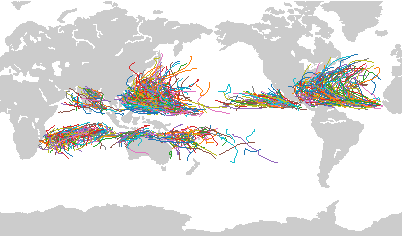
\includegraphics[width=\textwidth]{images/geomndp/storm/data_samples.pdf}
	\end{subfigure}
	\hfill
	\begin{subfigure}{.49\textwidth}
		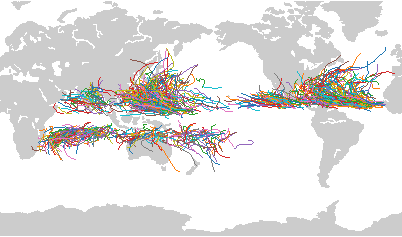
\includegraphics[width=\textwidth]{images/geomndp/storm/model_samples.pdf}
	\end{subfigure}
	\caption{\emph{Left:} 1000 samples from the training data. \emph{Right:} 1000 samples from the trained model.}
	\label{fig:cyclone_comparison}
\end{figure*}

\begin{figure*}[b!]
	\centering
	\begin{subfigure}{0.48\linewidth}
		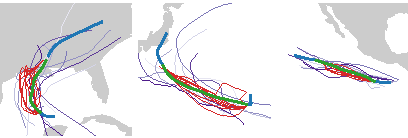
\includegraphics[width=\textwidth]{images/geomndp/storm/interpolation_examples.pdf}
		\caption{Interpolation}
	\end{subfigure}
	\hfill
	\begin{subfigure}{0.48\linewidth}
		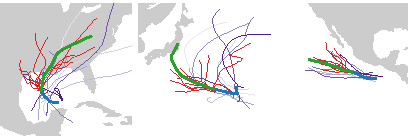
\includegraphics[width=\textwidth]{images/geomndp/storm/extrapolation_examples.pdf}
		\caption{Extrapolation}
	\end{subfigure}
	\caption{\emph{Top:}
		Examples of conditional trajectories sampled from the GeomNDP model.
		\emph{Blue:}
		Conditioned sections of the trajectory.
		\emph{Green:}
		The actual trajectory of the cyclone.
		\emph{Red:} conditional samples from the model. \emph{Purple:} closest matching trajectories in the dataset to the conditioning data.
	}
	\label{fig:interp_extrap_cyclone}
\end{figure*}
Finally, we assess our model on a task where the domain of the stochastic process is a non-Euclidean manifold.
We model the trajectories of cyclones over the earth, modelled as sample paths of the form \(\R \to \c{S}^2\) coming from a stochastic process.
The data is drawn from the International Best Track Archive for Climate Stewardship (IBTrACS) Project, Version 4 \cite{IBTrACSv4paper,IBTrACSv4data} and preprocessed as per \cref{sec:cyclonedetail}, where details on the implementation of the score function, the ODE/SDE solvers used for the sampling, and baseline methods can be found.

\Cref{fig:cyclone_comparison} shows some cyclone trajectories samples from the data process and from a trained \textsc{GeomNDP } model.
We also demonstrate how such trajectories can be interpolated or extrapolated using the conditional sampling method detailed in \cref{sec:conditional_sampling}.
Such conditional sample paths are shown in \cref{fig:interp_extrap_cyclone}.
Additionally, we report in \cref{tab:cyclone_results} the likelihood \footnote{We only report likelihoods of models defined with respect to the uniform measure on \(\mathcal{S}^2\).
}
and MSE for a series of methods.
We see that the GPs (modelled as \(f:\R\to\R^2\), one on latitude/longitude coordinates, the other via a stereographic projection, using a diagonal RBF kernel with hyperparameters fitted with maximum likelihood) fail drastically given the high non-Gaussianity of the data.
In the interpolation task, the \textsc{NDP} performs as well as the \textsc{GeomNDP }, but the additional geometric structure of modelling the outputs living on the sphere appears to significantly help for extrapolation.
See \cref{sec:cyclonedetail} for more fine-grained results.


\begin{table*}[t]
	\centering
	\small
	\begin{tabular}{lrrrrr}
		\toprule
		\multirow{2}{*}{\textsc{\textbf{Model}}}                  & \multicolumn{1}{c}{\textsc{Test data}} & \multicolumn{2}{c}{\textsc{Interpolation}} & \multicolumn{2}{c}{\textsc{Extrapolation}}                                                    \\
		                                                          & {Likelihood}                           & {Likelihood}                               & {MSE (km)}                                 & {Likelihood}           & {MSE (km)}              \\
		\midrule
		\rowcolor{pearDark!20} \textsc{GeomNDP  (\(\R\to\c{S}^2\))} & \(\mathbf{802_{\pm 5}}\)                 & \(\mathbf{535_{\pm 4}}\)                     & \(\mathbf{162_{\pm 6}}\)                     & \(\mathbf{536_{\pm 4}}\) & \(\mathbf{496_{\pm 14}}\) \\
		\textsc{Stereographic GP (\(\R \to \R^2/\{0\}\))}           & \(393_{\pm 3}\)                          & \(266_{\pm 3}\)                              & \(2619_{\pm 13}\)                            & \(245_{\pm 2}\)          & \(6587_{\pm 55}\)         \\
		\textsc{NDP (\(\R\to\R^2\))}                                & -                                      & -                                          & \({166_{\pm 22}}\)                           & -                      & \(769_{\pm 48}\)          \\
		\textsc{GP (\(\R\to\R^2\))}                                 & -                                      & -                                          & \(6852_{\pm 41}\)                            & -                      & \(8138_{\pm 87}\)         \\
		\bottomrule
	\end{tabular}
	\caption{
		Comparative results of different models on the cyclone dataset, comparing test set likelihood, interpolation likelihood and mean squared error, and extrapolation likelihood and mean squared error.
		Mean and std are estimated over 5 data splits / random seeds.
	}
	\label{tab:cyclone_results}
\end{table*}

\section{Discussion}
\label{sec:discussion}

In this chapter, we have extended diffusion models to model invariant stochastic processes over tensor fields.
We did so by \begin{enumerate*}[label=(\alph*)] \item constructing a continuous noising process over function spaces which correlate input samples with an equivariant kernel, \item parameterising the score with an equivariant neural network.
\end{enumerate*}
We have empirically demonstrated the ability of our introduced model {\scshape GeomNDP } to fit complex stochastic processes, and by encoding the symmetry of the problem at hand, we show that it is more data efficient and better able to generalise.

We highlight below some current limitations and important research directions.
First, evaluating the model is slow as it relies on costly SDE or ODE solvers.
In that respect our model shares this limitation with existing diffusion models.
Second, targeting a white noise process appears to over-perform other Gaussian processes.
In future work, we would like to investigate the practical influence of different kernels.
Third, we wish to apply our method for modelling higher order tensors, such as moment of inertia in classical mechanics~\parencite{thomas2018tensor} or curvature tensor in general relativity.
Fourth, strict invariance may sometimes be too strong, we thus suggest softening it by amortising the score network over extra spatial information available from the problem at hand.
